\documentclass[utf8]{gradu3}

\usepackage{graphicx}
\usepackage{amsmath}
\usepackage{booktabs}
\usepackage[backend=biber]{biblatex}
\usepackage[dvipsnames]{xcolor}

% HUOM! Tämän tulee olla viimeinen \usepackage koko dokumentissa!
\usepackage[bookmarksopen,bookmarksnumbered,linktocpage]{hyperref}

\addbibresource{gradubibtex.bib}

\begin{document}

\title{Avusteisen kommunikaation ohjelmiston toteuttaminen progressiivisena WWW-sovelluksena}
\translatedtitle{Augmentative and Alternative Communication Through a Progressive Web Application}
\studyline{Ohjelmistotekniikka}
\avainsanat{%
  Ionic,
  progressiiviset WWW-sovellukset,
  Angular,
  TypeScript,
  avusteinen kommunikaatio,
  autismi,
  käytettävyys
}
\keywords{%
  Ionic,
  progressive web applications,
  Angular,
  TypeScript,
  augmentative and alternative communication,
  autism,
  usability
}
\tiivistelma{%
  Progressiiviset WWW-sovellukset ovat verrattain tuore, mutta nopeasti suosituksi noussut tapa kehittää ohjelmistoja erilaisiin tarpeisiin. Tässä pro gradu -työssä Ionic-ohjelmistokehyksellä kehitettyä progressiivista WWW-sovellusta käytettiin tutkimaan avusteisen kommunikaation vaatimuksia, haasteita ja erikoispiirteitä sekä ohjelmistoteknisestä, että käytettävyysnäkökulmasta. Lisäksi tämän suunnittelutieteellisen tutkimuksen myötä pyrittiin saamaan kehittäjille yleistä tietoa progressiivisten WWW-sovellusten rakenteesta ja ominaisuuksista.
}
\abstract{%
  Progressive web applications are a recent, but very popular way to create applications for different needs. In this master's thesis, a progressive web application developed with the Ionic framework was examined to understand the needs of augmentative and alternative communication. This was done from a software engineering and a usability viewpoint. In addition, this master's thesis offers general insights about the structure and features of progressive web applications.
}

\author{Roope Kivioja}
\contactinformation{\texttt{roope.kivioja@gmail.com}}

\supervisor{Jonne Itkonen}
\supervisor{Jukka-Pekka Santanen}

\maketitle

\begin{thetermlist}
\item[\textbf{Ionic}] 

Mobiililaitteille suunniteltujen progressiivisten WWW-sovellusten kehittämiseen tarkoitettu avoimen lähdekoodin ohjelmistokehys.

\item[\textbf{Angular}] 

Googlen ylläpitämä avoimen lähdekoodin TypeScript-ohjelmistokehys.

\item[\textbf{TypeScript}] 

Microsoftin ylläpitämä avoimen lähdekoodin ohjelmointikieli.

\item[\textbf{Avusteinen kommunikaatio}]

 Kommunikointia, jossa puhetta joko tukee tai korvaa jokin tekninen apuväline tai muu keino kuten viittomakieli.

\item[\textbf{Electron}] 

GitHubin ylläpitämä progressiivisten WWW-sovellusten kehittämiseen tarkoitettu avoimen lähdekoodin ohjelmistokehys.

\end{thetermlist}

\mainmatter

\chapter{Johdanto}

Sosiaalinen kanssakäyminen on ihmisen perustarve ja jokaisella ihmisellä on sisäsyntyinen tarve tulla nähdyksi ja huomioiduksi. Ihmisillä on useita eri tapoja viestiä tahdollisesti ja tahtomattaan muiden ympärillään olevien ihmisten kanssa. Sosiaalisuus ja yhteistyö ovat ihmislajin määrittävimpiä tekijöitä. Siksi puhekyvyn menettäminen tai ilman sitä koko elämän eläminen on hyvin suuri haaste ihmisen elämässä. Teknologialla kuitenkin voidaan merkittävästi helpottaa tästä vaikeasta ongelmasta kärsivien ihmisten elämää.

Tässä pro gradu -työssä tutkitaan progressiivisia WWW-sovelluksia, avusteista kommunikaatiota ja niiden yhteensovittamista. Aihepiiriä ei juurikaan ole aiemmin tutkittu, joten suunnittelutieteellinen tutkimus valikoitui sen takia tämän pro gradu -työn tutkimustyypiksi. Tutkimustietoa kerättiin varsin paljon muiden kuin tietoteknisten julkaisujen aihepiiristä ja sitä jatkojalostettiin tämän tutkimuksen avulla ohjelmistotekniikan käyttötarpeisiin.

Idea tähän pro gradu -työhön syntyi, kun osallistuin Keski-Suomen Autismiliiton kokoontumisen järjestämiseen vuonna 2015. Vapaamuotoisessa kokoontumisessa pääsin näkemään miten autistiset nuoret käyttävät erilaisia apuvälineitä muiden ihmisten kanssa kommunikointiin. Osa nuorista käytti kommunikointiin paperisia apuvälineitä sekä henkilökohtaisen avustajan tukea, mutta osa pystyi kommunikoimaan itsenäisesti tablettitietokoneen avulla. Käyttäjien mielestä avusteisen kommunikaation ohjelmistojen laadussa ja saatavuudessa eri laitteille kuitenkin oli vielä paljon parantamisen varaa.

Toinen tämän pro gradu -työn aiheeseen vaikuttanut tapahtuma oli Adafy Oy:lle tekemäni projekti, jossa käytin Ionic-ohjelmistokehystä. Tuosta projektista minulle jäi vahva tunne, että progressiivisten WWW-sovellusten suosio tulee lähivuosina kasvamaan ja ne ovat käyttökelpoinen tapa toteuttaa yksinkertaisia ohjelmistoja. Viime vuosina näin on myöskin käynyt, sillä erittäin suositut monialustaiset ohjelmistot kuten Visual Studio Code, Slack ja Discord ovat kaikki Electron-ohjelmistokehyksen päälle rakennettuja.

\chapter{Tutkimuksen taustat}

Pro gradu -työn tavoitteena oli suunnittelutieteellisen tutkimuksen (engl. \textit{design study}) avulla muodostaa kuva progressiivisten WWW-sovellusten ja Ionic-kehyksen nykytilasta, eduista ja haasteista. Lisäksi tutkimuksessa perehdyttiin avusteiseen kommunikaatioon ja avusteisen kommunikaation mobiilisovellusten kehittämiseen sekä ohjelmistoteknisestä, että käytettävyysnäkökulmasta. Käytettävyystutkimuksessa otettiin huomioon erityisryhmien tarpeet ja etenkin autististen käyttäjien käytettävyyshaasteet.

Suunnittelutieteellisessä tutkimuksessa tutkimuksen kohteena ovat ihmisen tuotokset eli artefaktit. Suunnittelutieteellisessä tutkimuksessa arvioidaan palvelevatko artefaktit niille asetettuja tarkoituksia, ovatko ne hyödyllisiä ja toimivia sekä miten ne vertautuvat muihin artefakteihin. Suunnittelutieteellinen tutkimus on täten soveltavaa tutkimusta.

Tutkielmaa varten luotiin suunnittelutieteellisen tutkimuksen periaatteiden mukaisesti artefakti, \textbf{FreeAAC-ohjelmisto}. FreeAAC-ohjelmistolle asetettiin olemassa olevan tutkimuksen perusteella avusteiseen kommunikaatioon liittyviä ohjelmistoteknisiä ja käytettävyystieteellisiä tavoitteita. Näitä täydennettiin yleisillä ohjelmistoteknisillä ja käytettävyyspohjaisilla laatuvaatimuksilla. Tavoitteiden ja laatuvaatimusten perusteella pyrittiin lopuksi arvioimaan toteutuneen artefaktin ominaisuuksia.

Pro gradu -työn kohderyhmänä olivat sekä kehittäjät, että loppukäyttäjät. Kehittäjien näkökulmasta työssä keskeisiä tarpeita ja tavoitteita oli saada tietoa siitä miten Ionic-ohjelmistokehys soveltuu kommunikointisovelluksen kehittämiseen, sekä saamaan selville miten progressiiviset WWW-sovellukset rakentuvat ja mitkä ovat niiden etuja ja haasteita. Loppukäyttäjien eli autismin takia avustettua kommunikaatiota tarvitsevien henkilöiden näkökulmasta keskeinen tarve oli selvittää, mitä laatutekijöitä avusteisen kommunikaation ohjelmistoihin liittyy ja miten hyvin nämä laatutekijät pystytään toteuttamaan progressiivisen WWW-sovelluksen avulla.

Tutkimustyypin mukaisen selvitystyön ja näiden kahden ryhmän tarpeiden perusteella johdettiin joukko tavoitteita. Työssä haluttiin selvittää avusteisen kommunikaation ohjelmiston toiminnallisten ja käytettävyyden laatutekijät lähdemateriaalin perusteella. Näiden laatutekijöiden pohjalta muodostettiin joukko vaatimuksia, joiden pohjalta kehitettiin ohjelmisto ja pyrittiin arvioimaan sitä sekä rakenteellisesti, että edellä mainttujen laatutekijöiden ja vaatimusten toteutumiseen. Lisäksi haluttiin selvittää miten hyvin Ionic-ohjelmistokehys yleisesti sopii progressiivisten WWW-sovellusten kehittämiseen.

Pro gradu -työn ulkopuolelle rajattiin varsinainen käyttäjätutkimus sekä vertaileva tutkimus muihin tarjolla oleviin avusteisen kommunikaation ohjelmistoihin. Aikarajoitteiden vuoksi ohjelmistosta toteutettiin vain prototyyppiversio, joten käyttäjätutkimuksen toteuttaminen keskeneräisen ohjelmiston pohjalta olisi ollut haastavaa. Lisäksi autististen koekäyttäjien kanssa toiminen vaatii erikoisjärjestelyjä, jotka haluttiin rajata tämän työn ulkopuolelle. Prototyyppi-vaiheessa olevan ohjelmiston vertailu muihin tarjolla oleviin valmiisiin kaupallisiin ohjelmistoihin ei olisi tuottanut riittävän tarkkoja tuloksia johtopäätösten tekemiseen.

\chapter{Kommunikointisovelluksen rakentamiseen tarvittavia taustatietoja ja menetelmiä}

Avusteisen kommunikaation ohjelmiston suunnitteluun ja kehittämiseen tarvitaan perustietämystä kommunikaation haasteista kärsivien ihmisten tarpeista. Aihepiiri on monimutkainen ja useasti yksilökohtaisten vaatimusten sävyttämä, mutta olemassa olevan tutkimuksen pohjalta voidaan kuitenkin muodostaa joukko yleisiä vaatimuksia FreeAAC-ohjelmistolle.

\section{Avusteinen kommunikaatio}

On olemassa useita eri sairauksia ja kehityshäiriöitä, joiden johdosta henkilön kyky muodostaa puhetta voi hetkellisesti tai pysyvästi heikentyä. Puheen muodostamisen ongelmista kärsivä henkilö saattaa joutua turvautumaan arkipäivän kommunikaatiossa erilaisiin apuvälineisiin kommunikoidakseen muiden ihmisten kanssa. Yleisesti näitä viestintämenetelmiä kuvaamaan tarkoitettu termi on \textbf{puhetta tukeva ja korvaava kommunikaatio} (engl. \textit{Augmentative and Alternative Communication, lyh. AAC}).

Puhetta tukeva ja korvaava kommunikaatio voidaan jakaa kahtia: avustamattomaan ja avusteiseen. \textbf{Avustamattomalla puhetta tukevalla ja korvaavalla kommunikaatiolla} tarkoitetaan kommunikaatiota, jossa ei tarvita apuvälineitä. Viittomakieli on yksi esimerkki avustamattomasta puhetta tukevasta ja korvaavasta kommunikaatiosta, mutta myös ihmisen elekieltä voidaan pitää avustamattomana puhetta tukevana ja korvaavana kommunikaationa. 

\textbf{Avustettu puhetta tukeva ja korvaava kommunikaatio} tarkoittaa puolestaan kommunikaatiota, jossa käytetään jotain apuvälinettä. Apuvälineenä voi olla esimerkiksi valokuvia, kommunikaatiotaulu tai elektroninen laite. Tämän perusteella avustettu puhetta tukeva ja korvaava kommunikaatio voidaan jakaa edelleen kahdeksi ryhmäksi: matalan teknologian ja korkean teknologian puhetta tukevaan ja korvaavaan kommunikaatioon. Käyttäjä ei välttämättä käytä vain yhtä edellä mainituista tyypeistä. \parencite[]{AAC-conditional-use}

Puhetta tukevaa ja korvaavaa kommunikaatiota voidaan tarjota puheen muodostamisen ongelmista kärsiville myös tietoteknisten sovellusten avulla, joiden kautta käyttäjä kirjoittaa joko suoraan tekstiä tai kommunikoi valitsemalla symboleja. Esimerkiksi autistisilla käyttäjillä on tyypillisesti hyvin henkilö- ja yksityiskohtaisia tarpeita puhetta tukevalle ja korvaavalle kommunikaatiolle, joten tietoteknisten sovellusten suhteellisen helppo muokattavuus puoltaa niiden käyttöä perinteisempien puhetta ja kommunikointia korvaavien apuvälineiden sijaan.

\label{AAC-symbols}
Puhetta tukevat ja korvaavat kommunikointisovellukset käyttävät yleisimmin symboleja. Usein symbolit ryhmitellään kortteihin, joita on helppo vaihtaa tilanteeseen sopivaksi\label{AAC-cards}. Autisteille tyypillistä on vahva visuaalis-avaruudellinen hahmotuskyky, joten tutkimuksen mukaan piirroksiin ja valokuviin liitetyt merkitykset ovat tälle ryhmälle luonteva tapa kommunikoida. Vaughnin ja Hornerin tutkimuksessa \parencite[]{concrete-versus-verbal} Karl-nimisen autistisen koehenkilön haastava käytös ja aggressio vähenivät, kun pelkästään verbaalisesti annettujen ruokavaihtoehtojen rinnalle tuotiin kuvat ruoka-annoksista. Symbolipohjaiselle puhetta tukevalle ja korvaavalle kommunikaatiolle on siis sekä tutkimuspohjaista näyttöä että käytännön kokemuksiin perustuvaa kannustetta.

Puhetta tukevaan ja korvaavaan kommunikointisovellukseen voidaan liittää myös symboleita lukeva ääniominaisuus. Ääniominaisuus mahdollistaa kommunikoinnin näköyhteyden ulkopuolelle, vähentää symbolien tulkitsijan läsnäolon pakollisuutta ja helpottaa pidempien viestien rakentamista puhetta tukevassa ja korvaavassa kommunikointisovelluksessa. \parencite[]{AAC-interventions}

Ääniominaisuuden lisäämisellä avustetusta puhetta tukevasta ja korvaavasta kommunikaatiosta voidaan tehdä \textbf{monimodaalista} (engl. \textit{multimodal}). Monimodaalisuus tarkoittaa usean eri kommunikaatiotavan kautta tapahtuvaa kommunikaatiota. Monimodaalinen kommunikaatio voi tapahtua eri tapojen kautta yhtäaikaisesti tai peräkkäin. Puhetta tukevasta ja korvaavasta kommunikaatiosta kannattaa tehdä monimodaalista useista eri syistä. Ensinnäkin suurin osa kaikesta kommunikaatiosta on monimodaalista, sillä toiselle ihmiselle puhuttaessa on tavallista selkeyttää sanomaa ilmein ja elein. Toiseksi puhetta tukevaa ja korvaavaa kommunikaatiota käyttävä henkilön tulee useasti kommunikoida muiden puhetta tukevaa ja korvaavaa kommunikaatiota käyttävien henkilöiden kanssa, jolloin vaihtoehdoista on hyötyä. Kolmas merkittävä syy on se, että eri puhetta tukevissa ja korvaavissa kommuunikaatiotavoissa on vahvuuksia ja heikkouksia, joten eri kommunikaatiotapoja sekoittamalla voidaan korvata yksittäisen kommunikaatiotavan heikkouksia. \parencite[]{AAC-conditional-use}

Puhetta tukevaan ja korvaavaan kommunikaatioon liittyy useita haasteita. Koska syyt ja tarpeet puhetta korvaavalle kommunikaatiolle ovat hyvin moninaisia, yhtenäisiä käytäntöjä on vaikea muodostaa ja tarve henkilökohtaiselle räätälöinnille on suurta. Lisäksi puhetta tukevaa ja korvaavaa kommunikaatiota tarvitsevien henkilöiden määrä ei ole väestötasolla kovin suuri. \colorbox{YellowGreen}{// TODO: lähde?} Tämän takia puhetta tukevia ja korvaavien kommunikointisovellusten tuottamiseen on hyvin vähän kaupallista kannustetta.

\section{Progressiiviset WWW-sovellukset}

\textbf{Progressiiviset sovellukset} (engl. \textit{Progressive Web Applications, lyh. PWAs}) ovat selaimessa ajettavia WWW-sovelluksia, joiden ulkoasu määrittyy alustakohtaisesti niin, että niiden ulkoasu on mahdollisimman yhdenmukainen laitteen natiivien sovellusten kanssa. Selainpohjaisuuden takia progressiiviset sovellukset pystyvät käyttämään tarjolla olevia sovellusympäristön resursseja joustavasti sen sijaan, että ne itse määrittäisivät vaatimukset toiminnalleen. Termi on verrattain tuore ja vakiintumaton, sillä esimerkiksi Ionic-kehyksen dokumentaatiossa käytetään myös termiä \textbf{hybridisovellus} (engl. \textit{hybrid application}).

Progressiivisten sovellusten ilmeisin hyöty on alustariippumattomuus. Samaa sovellusta voidaan käyttää kaikissa ympäristöissä, jotka tukevat moderneja WWW-selaimia. Eri versioita samasta sovelluksesta ei tarvitse kehittää ja ylläpitää erikseen, joten progressiivisten sovellusten avulla voidaan säästää kalliita työresursseja. Hyvä esimerkki progressiivisten sovellusten käyttöä tukevasta markkinatilanteesta on nykyisten älytelevisioiden kirjava tarjonta, sillä valmistajien omien käyttöjärjestelmien lisäksi muunmuassa Apple, Amazon ja Roku kehittävät televisioon liitettäviä laitteita, joiden avulla käyttäjä voi ajaa erilaisia sovelluksia. Näiden kaikkien laitteiden tukeminen olisi hyvin vaikeaa perinteisten sovellusten avulla. \parencite[]{frankston-pwa}

Tällä hetkellä erityisesti Google panostaa progressiivisten sovellusten kehittämiseen Chrome-selaimen kehitysympäristön yhteydessä. Googlen \parencite[]{google-pwa-marketing} mukaan progressiiviset sovellukset tarjoavat perinteisiin WWW-sovelluksiin verrattuna enemmän luotettavuutta, käytettävyyttä ja monipuolisempaa sisältöä. Yrityksen mukaan luotettavuus paranee, sillä progressiiviset sovellukset pystyvät tarjoamaan sisältöä myös ilman verkkoyhteyttä. Google myös väittää, että progressiivisten sovellusten kohdalla käytettävyyttä parantaa nopeammin käyttäjän komentoihin vastaava käyttöliittymä ja sovellusmaisuus puolestaan parantaa käyttäjän immersiota.

Googlen Chrome-selain on rakennettu avoimen lähdekoodin Chromium-selaimen päälle. Yksi merkittävimmistä Chromium-selaimeen pohjautuvista progressiivisten WWW-sovellusten kehitykseen tarkoitetuista kehyksistä on Electron. Electron on Microsoftin nykyisin omistaman GitHubin kehittämä ja ylläpitämä. Esimerkkejä Electron-sovelluksista ovat Discord, Slack ja Visual Studio Code. Microsoftin päätös muuttaa Edge-selain Chromium-pohjaiseksi saattoi johtua ainakin osittain progressiivisten WWW-sovellusten vaatimista ominaisuuksista kuten tehokkaammasta muistinhallinnasta.

Twitter, AliExpress ja Lancôme ottivat vuonna 2017 käyttöön progressiiviset sovellukset ja julkaistut tulokset ovat olleet positiivisia. Twitter onnistui uuden progressiivisen sovelluksensa ansiosta lisäämään sivupäivityksiä 65\% käyttäjäsessiota kohden, lisäämään lähetettyjen Twitter-viestien määrää 75\% ja vähentämään käytön lopettamista 20\%. Lisäksi uusi sovellus käytti vähemmän kuin 3\% natiivin sovelluksen vaatimasta muistitilasta ja vähensi datan käyttöä 70\%. Datan käytön määrän vähentyminen on erityisen merkittävää, koska Twitter arvioi, että vuonna 2017 45\% sen sisällöstä ladattiin 2G-verkon läpi. \parencite[]{beginners-guide-pwa}   
\colorbox{YellowGreen}{// TODO: Kriittisempi ote.}

AliExpress ja Lancôme ovat molemmat verkkokauppoja, joilla on ollut ongelmia mobiiliverkkokauppojensa tehokkuuden kanssa. Progressiiviseen sovellukseen siirtymällä AliExpress lisäsi uusien asiakkaiden myyntitapahtumien määrää 104\%:lla ja Lancôme 17\%:lla. Lisäksi AliExpress tuplasi sivunlatausten määrän sekä kasvatti sessioiden pituutta 74\%:lla. Lancôme puolestaan onnistui lisäämään iOS-sessioiden määrää 53\%:lla. Edellä mainitut tulokset eivät kuitenkaan ole suoraan yleistettävissä yleisemmin progressiivisten sovellusten vaikutuksiin, sillä niiden otoskoko on erittäin pieni. \parencite[]{beginners-guide-pwa}

Progressiivisten WWW-sovellusten käyttö ei kuitenkaan ole ongelmatonta. Ensinnäkin, koska progressiivisten WWW-sovellusten hyödyntämät teknologiset kehitysaskeleet ja niiden käyttöön kannustavat taloudelliset tekijät ovat verrattain tuoreita, vaaditaan kehittäjiltä paljon uusien asioiden opettelua sekä vakiintumattomien työkalujen ja kehysten käyttämistä kehitystyössä. Toinen merkittävä haaste voi olla tiedon tallentaminen, sillä selaimen toimintaan pohjautuvalle sovellukselle ei ole varattu tietoturvan takia samoja oikeuksia kuin natiiveille sovelluksille. Kolmas ongelma voi tulla eteen käytettävyydessä, sillä selaimessa toimivan sovelluksen vaatimat resurssit saattavat hidastaa sovelluksen toimintaa. \parencite[]{pwa-design-challenges}

Myös progressiivisten sovellusten keskusmuistinkäyttöä on kritisoitu. Progressiiviset sovellukset vaativat perinteisiä sovelluksia enemmän muistia, koska niitä ajetaan selaimen päällä. On vaikea arvioida, kuinka suuri osa muistinkäytöstä johtuu sovelluksen toteutuksesta ja kuinka suuri osa itse ohjelmistokehyksestä, mutta hyvin yksinkertaisissakin testeissä on saatu tuloksia, jotka viittaavat moninkertaiseen keskusmuistinkäyttöön natiiveihin sovelluksiin verrattuna \parencite[]{electron-memory-usage}.
  
\colorbox{YellowGreen}{// TODO: selaimen päällä on puhekielisyys}

Suuremman muistinkäytön lisäksi myös energiankulutus saattaa olla korkeampi progressiivissa WWW-sovelluksissa. Ohjelmistoanalyyttiikkatyökalua tarjoavan Greenspectorin mukaan \parencite[]{pwa-power-usage} Twitterin progressiivisen WWW-sovelluksen energiankulutus valmiustilassa on 12-25\% korkeampi asetuksista riippuen. Greenspectorin motiivit saattavat kuitenkin olla ristiriidassa puolueettoman ohjelmistoanalyysin kanssa, joten tulokset eivät ole välttämättä täysin luotettavia. Voidaan kuitenkin olettaa, että ainakin lisääntynyt muistinkäyttö aiheuttaa myös lisääntynyttä energiankulutusta ja täten haittaa mobiililaitteiden pitkäaikaista käyttöä.

Progressiiviset WWW-sovellukset sopivat siis parhaiten tilanteisiin, joissa vähän muistia vaativan sovelluksen halutaan tukevan useita eri alustoja, mutta joissa tavallinen WWW-sivu ei riitä. Avusteisen kommunikaation sovelluksien vaatimukset osuvat hyvin yhteen progressiivisten WWW-sovellusten vaatimusten kanssa, sillä kuvakorttien näyttäminen ei ole muisti-intensiivistä, mutta toisaalta taas avusteisen kommunikaation sovellusten halutaan olevan helposti muovattavissa henkilökohtaisiin tarpeisiin sopiviksi sekä toimivan useilla eri alustoilla.

\section{Ionic-ohjelmistokehyksen rakenne ja ominaisuudet}

Ionic on yksi suosituimpia progressiivisten sovellusten kehittämiseen tarkoitetuista ohjelmistokehyksistä. \colorbox{YellowGreen}{// TODO: Lähde} Electronin ollessa työasemille suunnattu kehys, Ionic keskittyy mobiililaitteiden vaatimuksiin. Ionic on avointa lähdekoodia ja hyödyntää Apache Cordova -ympäristöä sekä suosituimpia frontend-ohjelmistokehyksiä. Aiemmin Ionic tuki vain Angular-ohjelmistokehystä, mutta Ionicin versiosta 4 lähtien kehittäjällä on mahdollisuus valita itse käyttämänsä frontend-kehys. Ionic on MIT-lisenssin alainen ja täten avointa lähdekoodia. Angular-ohjelmistokehys perustuu TypeScript-ohjelmointikieleen. Ionicin perusrakenne on kuvattuna kaaviossa \ref{fig:ionic-structure}. Ohjelmistokehyksenä Ionicin päämäärä on tarjota kehittäjälle oikealta näyttävä ja visuaalisesti toimiva sovellus. Sen ei ole tarkoitus korvata tyypillisiä JavaScript-kirjastoja, vaan se toimii niiden tukena. \parencite[]{ionic-documentation}

\begin{figure}[h]\centering
  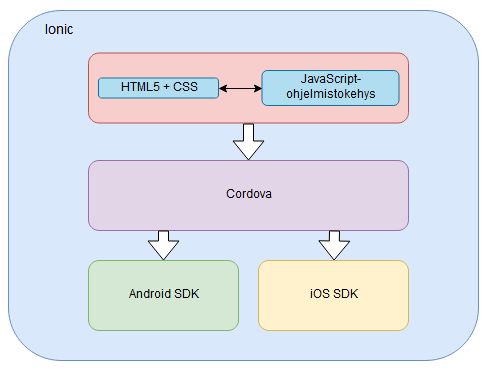
\includegraphics[height=9cm,keepaspectratio]{ionic-structure}
  \caption[Ionic-sovelluksen perusrakenne]
  {Ionic-sovelluksen perusrakenne.}
  \label{fig:ionic-structure}
\end{figure}

Ionicia ylläpitää ja kehittää Ben Sperryn ja Max Lynchin perustama samanniminen yritys. Avoimen lähdekoodin projektina Ionic-kehyksen kehitykseen ja ylläpitoon pääsee osallistumaan GitHub-sivuston välityksellä kuka tahansa. Ionicin viimeisin pääversio on 4.0.0. Viime aikoina Ionicin kehitystyössä painoarvoa on annettu erityisesti Ionic-kehyksen ja Angularin välisten riippuvuuksien vähentämiseen, jotta Ionicia voitaisiin käyttää muiden kehyksien kuten Reactin ja Vue.js:n yhteydessä.

Ionic koostuu komponenteista. Ionicin komponentit ovat uudelleenkäytettäviä käyttöliittymäelementtejä, jotka toimivat sovelluksen käyttöliittymän rakennusosina. Niiden avulla sovellus näyttää yhtenäiseltä ja käyttöliittymän kehitystyö nopeutuu. Komponentit koostuvat HTML:stä, CSS:stä ja JavaScriptistä. Esimerkkejä tällaisista komponenteista ovat muunmuassa painikkeet, välilehdet ja erilaiset listat. Ionicin toteutuksessa on pyritty tukemaan näiden komponenttien mahdollisimman joustavaa räätälöintiä \parencite[]{ionic-documentation}.

Ionicin ulkoasu perustuu teemoihin. Myös teemat lisäävät sovelluksen ulkoasun yhtenäisyyttä. Teemat myös mukautuvat eri alustojen ulkoasustandardien mukaisiksi kehittäjän niin halutessa. Esimerkiksi Android- ja iOS-mobiilikäyttöjärjestelmille suunnattujen sovellusten ulkoasu poikkeaa toisistaan, jos käytetään Ionicin oletusteemoja. Teemojen käyttäminen parantaa sovelluksen käytettävyyttä tekemällä sen ulkoasusta ennustettavamman ja tutumman loppukäyttäjälle. Ionicin oletusteemat noudattavat Applen iOS-designperiaatteita \parencite[]{ios-design-guide} sekä Googlen Material Design -määrityksiä \parencite[]{google-material-design}.

\subsection{Apache Cordova}

Apache Cordova (aikaisemmin PhoneGap) on alunperin Nitobin kehittämä sovelluskehitysympäristö mobiililaitteille. Adobe osti Nitobin vuonna 2011 ja myöhemmin uudelleenjulkaisi Apache Cordovan avoimena lähdekoodina. Apache Cordova toimii WWW-sovelluskehyksien ja natiivien sovelluskehyksien välisenä linkityskerroksena \parencite[]{ionic-framework-hybrid}. Apache Cordovan avulla Ionic ja muut Apache Cordovan päälle rakennetut ohjelmistokehykset voivat toimia syvemmällä tasolla kuin tyypillinen WWW-sovellus, sillä niille tarjoutuu rajapinta suoraan natiiveihin sovelluskehyksiin. Näin progressiivisille WWW-sovelluksille tarjoutuu mahdollisuus käyttää muunmuassa mobiililaitteen kameraa ja GPS-paikannusta.

\subsection{Angular}

Angular on Googlen Angular Teamin ylläpitämä TypeScript-pohjainen käyttöliittymäkehys. Se on jatkoa aiemmin ilmestyneelle AngularJS-kehykselle. Alkuperäinen AngularJS-kehys julkistettiin vuonna 2010, ja se oli ensimmäinen suosittu ohjelmistokehys dynaamisten HTML-sivujen kehittämiseen mahdollistaen tehokkaamman yhden sivun WWW-sovellusten rakentamisen. Angular julkaistiin vuonna 2016, ja se on kokonaan uudelleenohjelmoitu versio AngularJS:stä.

AngularJS perustuu MVC-arkkitehtuuriin, kun taas uudempi Angular on komponenttipohjainen. Komponenttipohjainen arkkitehtuuri pyrkii tarjoamaan paremman uudelleenkäytettävyyden, luettavuuden, testattavuuden ja ylläpidettävyyden. Ohjelma jaetaan itsenäisiin komponentteihin, joita voidaan käyttää useasti ja niiden itsenäisyys helpottaa yksikkötestaamista. Itsenäiset komponentit ovat huomattavasti helpommin ymmärrettävissä ja niiden korvaaminen on joustavampaa, mikä parantaa ylläpidettävyyttä. \parencite[]{good-and-bad-angular} 

Angularin komponenttipohjainen rakenne perustuu kolmeen hiljattain ilmestyneeseen teknologiaan: Web-komponentteihin (engl. \textit{Web Components}), JavaScriptin ES2015-standardiin ja TypeScript-ohjelmointikieleen.

\textbf{Web-komponentit} on sateenvarjotermi, jolla tarkoitetaan neljää WWW-selaimissa yleistyvää standardia: kustomoitavat elementit (engl. \textit{custom elements}), varjo-dokumenttioliomalli (engl. \textit{shadow DOM}), mallit (engl. \textit{templates}) ja HTML-tuonti (engl. \textit{HTML imports}). 

\textbf{Kustomoitavat HTML-elementit} ovat HTML-standardielementtien ulkopuolisia elementtejä, joita voidaan käyttää standardielementtien seassa. Kustomoitava HTML-elementti irroittaa komponentin sivun muista osista, joten se mahdollistaa komponentin eristämisen. 

\textbf{Varjo-dokumenttioliomalli} on piiloitettu osa sivua, jolla on oma eristetty ympäristö skripteille, CSS-tyylitiedostoille ja HTML-elementeille. Varjo-dokumenttioliomallin elementit ja tyylit eivät vaikuta varjo-dokumenttioliomallin ulkopuolisiin alueisiin ja vastavuoroisesti muut sivun elementit ja tyylit eivät vaikuta varjo-dokumenttioliomallin alaisiin osiin. Tätä eristettyä aluetta voidaan täten käyttää komponentin piirtämiseen. 

\textbf{Mallit} ovat HTML-palasia, jotka eivät lataudu välittömästi HTML-sivun auetessa, vaan ne voidaan aktivoida JavaScriptillä myöhemmin. Malleista on useita toteutuksia eri kehyksissä, mutta Web-komponentit standardisoivat mallien rakentamisen ja tarjoavat suoran tuen niiden hyödyntämiselle selaimessa. Malleja käyttämällä varjo-dokumenttioliomalliin piilotetusta sisällöstä voidaan tehdä dynaamista. 

Viimeinen Web-komponenttien osa on \textbf{HTML-tuonti}. HTML-tuonnin avulla HTML-, CSS- ja JavaScript-tiedostoja voidaan ladata yhtenäisinä osina. Angular ei käytä HTML-tuontia, vaan se käyttää JavaScriptin moduulilatausta. \parencite[]{angular-6-by-example}

\subsection{TypeScript}

TypeScript on avoimen lähdekoodin ohjelmointikieli, jota ylläpitää Microsoft. TypeScript kääntyy suoritusvaiheessa JavaScriptiksi, ja se on tarkoitettu tukemaan JavaScript-ohjelmien kehitystä parantelemalla JavaScriptin ominaisuuksia. TypeScript sisältää ES 2015 -standardin mukaiset ominaisuudet sekä lisäksi se tarjoaa ohjelmoijan käyttöön tyypit ja koristelijat. Angular-ohjelmointikehyksen ohjelmointiin käytetään TypeScript-ohjelmointikieltä.

TypeScriptin on tarkoitus tarjota Microsoftin .NET-ympäristöön tottuneille ohjelmoijille oliolähtöisempi lähestymistapa JavaScript-kehitykseen \parencite[]{maharry-typescript}. JavaScript on suosittu ohjelmointikieli, mutta varsinkin ohjelmiston lähdekoodin määrän kasvaessa sen heikkoudet alkavat tulla esiin. TypeScript pyrkii puuttumaan näihin ongelmiin tarjoamalla ohjelmoijalle moduulijärjestelmän, luokat, rajapinnat ja staattisen tyypityksen \parencite[]{understanding-typescript}.

Ohjelmointikielen \textbf{modulaarisuudella} viitataan yleisesti itsenäisistä osista kasattaviin suurempiin kokonaisuuksiin. TypeScriptissä modulaarisuus on toteutettu siten, että muuttujat, funktiot, luokat ja muut vastaavat ohjelmointikielen perusrakenteet ovat olemassa vain moduulien sisällä, ellei niitä erikseen esitellä muille moduuleille \parencite[]{typescript-modules}. Tämä vähentää ohjelman eri osien välistä riippuvuutta toisistaan, mikä helpottaa muutosten tekemistä ohjelmistoon.

Perinteisesti JavaScript on käyttänyt uudestikäytettävien komponenttien rakentamiseen funktioita ja prototyyppipohjaista perintää. Iso osa nykyohjelmoijista ei kuitenkaan ole tottunut käyttämään edellä mainittuja keinoja, vaan nykyisin suosituin lähestymistapa uudelleenkäytettävyyteen on luokkien käyttäminen. Myös JavaScriptin oliotukea on pyritty parantelemaan sen viimeisimmissä versioissa. \parencite[]{typescript-classes}

Uudelleenkäytettävyyden lisäksi TypeScriptin luokkien avulla saadaan aikaan modulaarisia komponentteja, joita on helpompi ylläpitää ja skaalata. Virheiden löytämistä helpottaa se, että luokkien avulla ohjelmakoodin rajoista saadaan selkeämpiä. Skaalautuvuutta varten täytyy monesti pystyä korvaamaan vanhoja komponentteja uusilla ja luokkia käyttämällä myös tämä on helpompaa.

\textbf{Rajapintoja} käytetään kuvaamaan luokkien ominaisuuksia. TypeScriptissä rajapintoja käytetään tyyppien nimeämiseen ja niiden avulla voidaan tehdä olioiden välisiä sopimuksia ohjelmoijan itse laatiman ohjelmistokoodin sisällä sekä myös ohjelmoijan oman ohjelmistokoodin ja muiden kehittämien kirjastojen välillä. \parencite[]{typescript-interfaces} Esimerkiksi Swagger-niminen työkalu generoi .NET-palvelinkoodista valmiita rajapintoja, joita TypeScript-pohjaisen WWW-sovelluksen on helpompi käyttää. Rajapinnat ovat luonnollinen osa luokkiin perustuvaa ohjelmointia. Niiden avulla luokan toteutus voidaan eroittaa sen ulkopuolelle näkyvistä osista ja jakaa luokkia ryhmiin. Kuten luokkienkin kohdalla, rajapintojen käyttäminen voi parantaa ohjelman ylläpidettävyyttä, skaalautuvuutta ja osien uudelleenkäytettävyyttä.

JavaScriptistä poiketen TypeScript on staattisesti tyypitetty kieli. Tyypitys tarkoittaa sitä, että muuttujien ja olioiden tyypit täytyy määritellä ohjelmakoodissa. Dynaamisesti tyypitetyissä kielissä kuten JavaScriptissä muuttujien tyypit päätellään käännöksen aikana. Staattisen tyypityksen avulla ohjelmoijan on helpompi nähdä suoraan, että ohjelman tieto on oikean tyyppistä sitä käsitellessä. Iso osa tyyppivirheistä jää tällöin kiinni jo ennen kääntämistä kun taas JavaScriptilla ohjelmoidun ohjelman kohdalla näin ei käy. Toisaalta vahva tyypitys aiheuttaa lisätyötä tyyppimuunnosten takia.

\section{Käytettävyyden perusteet}
\colorbox{YellowGreen}{// TODO: Parempi nimi luvulle?}

Kaikkiin ihmisen tuottamiin esineisiin ja asiohin liittyy tiedostettu tai tiedostamaton suunnitteluprosessi. Vaikka ihmiset ovat suorittaneet aktiivista suunnittelua esihistoriallisista ajoista saakka, on tietoisten suunnitteluprosessien tutkimus verrattain tuoretta. \colorbox{YellowGreen}{// TODO: Täsmennä} Nykyinen suunnittelun kenttä voidaan jakaa karkeasti kolmeen eri osaan: teollinen suunnittelu, käytettävyyssuunnittelu ja kokemussuunnittelu \parencite[]{norman-doet}. Jokapäiväisessä kommunikaatiossa avustavan sovelluksen suunnittelussa tulee olla erityisen kiinnostuneita käytettävyyssuunnitelusta.

Hyvin suunniteltu sovellus on miellyttävä käyttää ja ohjaa käyttäjää käyttämään sovellusta oikealla tavalla. Tämä on erityisen tärkeää sovelluksissa, joita on tarkoitus käyttää arkisissa tilanteissa, jotka vaativat reaaliaikaista reagointia muiden ihmisten kommunikointiin. Avustettua kommunikaatiota käyttävillä ryhmillä on myös omia käytettävyystarpeita, joiden huomioimista varten täytyy ymmärtää käytettävyyttä tavallista laajemmassa kontekstissa.

\label{general-usability-requirements}
Ohjelman käyttöliittymän \textbf{käytettävyys} (engl. \textit{usability}) on laadullinen määre, joka \colorbox{YellowGreen}{// TODO: lähde} voidaan jakaa viiteen laadulliseen osa-alueeseen: opittavuus (engl. \textit{learnability}), tehokkuus (engl. \textit{efficiency}), muistettavuus (engl. \textit{memorability}), virhealttius (engl. \textit{errors}) ja tyydyttävyys (engl. \textit{satisfaction}).

\colorbox{YellowGreen}{// TODO: Jaa nämä kategoriat alla oleviin kappaleisiin}

\textbf{Opittavuus} tarkoittaa sitä miten helppo käyttöliittymää on oppia käyttämään. Käyttöliittymän \textbf{tehokkuus} määrittyy siitä miten nopeasti käyttäjät voivat suorittaa ohjelman toimintoja sen jälkeen kun ohjelman käyttöliittymää on opittu käyttämään. \textbf{Muistettavuus} on määre, jonka avulla arvioidaan miten nopeasti käyttäjä muistaa toiminnot ohjelman käyttämisen lopettamisen ja uudelleen aloittamisen jälkeen. \textbf{Virhealttiudella} tarkoitetaan käyttäjien tekemien virheiden määrää ja niiden laatua sekä kuinka helppoa niistä selviäminen on. \textbf{Tyydyttävyys} kertoo, miten tyytyväinen käyttäjä on käyttöliittymään. On olemassa muitakin laadullisia määreitä, kuten \textbf{käyttökelpoisuus} (engl. \textit{utility}), jolla määritellään ohjelman tarjoamien eri ominaisuuksien määrää ja vertaamista haluttuihin ominaisuuksiin. Käytettävyyttä ja käyttökelpoisuutta yhtä aikaa tarkistelemalla saadaan aikaan kuva ohjelman \textbf{hyödyllisyydestä} (engl. \textit{usefulness}). \parencite[]{usability-101}

Lyhyesti ilmaistuna, opittavuus tarkoittaa ohjelmiston kykyä opettaa käyttäjälleen oikea tapa käyttää ohjelmistoa. Opittavuutta vastaava termi on \textbf{löydettävyys} (engl. \textit{discoverability}). Opittavuutta lisääviä ominaisuuksia ovat muunmuassa muistettavuus, loogisuus, toistettavuus ja yhdenmukaisuus. Opittavuudeltaan hyvä ohjelma ilmaisee käyttäjälleen tehokkaasti mitä toiminnallisuuksia se sisältää, mitä eri toiminnot tarkoittavat ja kuinka eri toiminnallisuuksia käytetään. \parencite[]{improving-learnability}

Tehokkuus on määritelmä tai mitta sille, miten helposti ja nopeasti haluttu toiminto voidaan suorittaa tuttua käyttöliittymää käyttämällä. Tehokkuutta voidaan suoraan mitata esimerkiksi kulunutta aikaa tai välivaiheiden määrää mittaamalla. 

Muistettavuus mittaa sitä, miten helppo käyttäjän on käyttää ohjelmistoa sen jälkeen, kun ohjelmiston edellisestä käyttökerrasta on kulunut aikaa. Muistettavuutta on hankala mitata suoraan tyypillisten käyttäjätutkimusmetodien avulla, mutta esimerkiksi Affordable Usability -sivuston \parencite[]{affordable-usability} mukaan sitä voidaan WWW-sovellusten yhteydessä tutkia erilaisten verkkosivuanalytiikkatyökalujen avulla.

Käyttäjien tekemien virheiden määrän minimointi on yksi käyttettävyyssuunnittelun tärkeimmistä tavoitteista. Don Normanin \parencite[]{norman-doet} mukaan  käyttäjää ei juuri koskaan pitäisi syyttää tekemistään virheistä vaan suurin osa käyttövirheistä johtuu huonosta suunnittelusta.

Tyydyttävyys mittaa sitä miten hyvin käyttöliittymä ottaa huomioon käyttäjän tarpeet ja miten miellyttävää käyttö on. Tyydyttävyyttä ymmärtääkseen täytyy tietää, että käyttöliittymä ja käyttäjäkokemus ovat kaksi eri asiaa. Käyttäjäkokemus ja sen tyydyttävyys tai tyydyttämättömyys on seurausta useasta eri tekijästä. Visuaalinen ulkoasu on osatekijä käyttöliittymän tyydyttävyyttä arvioidessa, mutta myös halutuilla ominaisuuksilla ja niiden toimivuudella on merkitystä tyydyttävyyteen. Jos käyttäjä ei löydä haluamiaan toimintoja, osa halutuista ominaisuuksista puuttuu tai ne on hankalta löytää, ohjelmiston tyydyttävyys on matala. Tyydyttävyys on viidestä edellä listatusta käytettävyystekijästä kaikista subjektiivisin.

\subsection{Käytettävyys ja avusteinen kommunikaatio}

Avusteiseen kommunikaatioon liittyy omia käytettävyyshaasteita. Tarve avusteiseen kommunikaatioon voi johtua useista eri syistä, joten käyttäjäkirjo ja käyttäjien henkilökohtaisten tarpeiden määrä on suuri. Jo pelkästään tämän havainnon perusteella voidaan olettaa ohjelmiston muokattavuuden olevan tärkeää.

CP-vammaisten avusteista kommunikaatiota tutkineessa tutkimuksessa \parencite[]{classmate-aac-study} yksi merkittävä käytettävyystekijä on avusteista kommunikaatiota käyttävän henkilön hidas toiminta. Avusteista kommunikaatiota käyttävä henkilö ei välttämättä pysty reagoimaan nopeasti eri keskusteluaiheisiin tai muodostamaan riittävän paljon kommunikaatiota, jolloin keskustelukumppani joutuu arvaamaan, mitä avusteista kommunikaatiota käyttävä henkilö yrittää sanoa. Käytettävyyden näkökulmasta on myös huomioitava, että käyttäjällä on riittävästi aikaa suorittaa valintoja käyttöliittymässä ilman, että näkymä vaihtuu tai käyttöliittymäelementit muuttuvat.

\label{AAC-context-settings}
Comunicador-nimistä espanjankielisille avusteisen kommunikaation käyttäjille tarkoitettua ohjelmistoa käsittelevässä tutkimuksessa \parencite[]{graphic-communicator} nostetaan esiin kontekstiriippuvaisten valintojen tärkeys. Koska kommunikointi on usein vaivalloista avusteisten kommunikaation sovellusten kautta, avusteisen kommunikaation sovelluksessa on hyvä olla mahdollisuus ryhmitellä esivalmistellut sanat tai kuvat tilanteiden mukaan. Esimerkiksi työ-, harrastus- ja arkitilanteissa tarvitaan usein hyvin erilaisia sanavarastoja. Kontekstin valitsemisen lisäksi sanoja tai kuvia täytyy myös pystyä ryhmittelemään ja järjestelemään kontekstiryhmien sisällä.

\label{AAC-staticity}
Autismi vaikuttaa monella tapaa ihmisen kykyyn havainnoida ympäristöä ja sen myötä kykyyn käyttää sovelluksia. Iso-Britannian The National Autistic Society listaa verkkosivuillaan \parencite[]{autism-friendly-websites} autistisille ihmisille sopivien verkkosivujen visuaalisen toteutuksen päävaatimukset. Listauksessa painotetaan erityisesti visuaalisen ilmeen selkeyttä, staattisuutta ja yksiselitteisyyttä. Lisäksi koekäyttäjien roolia korostetaan.

Ilmaiseksi tarjolla olevia avusteisen kommunikaation mobiilisovelluksia tutkineen tutkimuksen \parencite[]{autism-mobile-usability} mukaan autistisilla käyttäjillä on ominaisuus- ja käytettävyystarpeita, joita tarjolla olleissa sovelluksissa ei ole. Tutkimuksen mukaan mahdollisuus kuvien ottamiseen sekä äänen tallentamiseen on erittäin hyödyllinen ominaisuus avusteisia kommunikaatiosovelluksia käyttäville autisteille. Kuvat eri sijainneista ja ihmisistä auttavat päivittäisessä kommunikaatiossa huomattavasti. \label{AAC-photos}

\label{AAC-settings}
Kommunikaatiosovelluksessa tulisi myös olla mahdollisuus säätää ohjelman asetuksia hallintapaneelin kautta. Hallintapaneelin tulisi olla salasanasuojattu, jotta käyttäjä ei pääse vahingossa poistamaan tärkeitä asetuksia tai kuvia sovelluksesta. Yhteen näyttöön ei saa mahduttaa liian paljon informaatiota, sillä autismiin liittyy usein aistiyliherkkyyttä \colorbox{YellowGreen}{// TODO: lähde}, mikä heikentää autistisen henkilön kykyä ymmärtää isoja määriä informaatiota kerrallaan. Tämän takia esimerkiksi kommunikaatiosovelluksen korteilla olevien kuvien määrää tulisi pystyä säätämään sovelluksen hallintapaneelista. \label{AAC-cardsize}

\label{AAC-soundsynth}
Kommunikaatiosovellusten ääniominaisuus voi auttaa käyttäjää oppimaan sovelluksen käyttöä nopeammin. Äänisyntetisaattoreita Martin-nimisen pojan avulla tutkineessa tutkimuksessa \parencite[]{voca-efficacy} havaittiin, että Martin oppi muodostamaan uusia lauseita helpommin, kun avusteisen kommunikaation sovellus luki kirjoitetun tekstin ääneen. Tutkimuksen luotettavuutta kuitenkin heikentää se, että tutkimuksessa tutkittiin vain yhden koehenkilön oppimistuloksia.

\label{symbol-libraries}
Symbolien käyttöä sovelluksien käyttöliittymissä tekstin korvikkeena pidetään yleisesti hyvänä tapana säästää tilaa, vähentää lukemisen aiheuttamaa kognitiivista kuormaa sekä kiertää tarvetta tekstien kääntämiseen useille eri kielille. Autistisilla henkilöillä esiintyy kuitenkin useasti hahmotusongelmia, jotka haittaavat symbolien merkityksen ymmärtämistä. Autististen henkilöiden on keskimäärin haastavaa ymmärtää abstraktien ja vähän ikonisuutta sisältävien symbolien merkitystä. \label{AAC-abstract-symbols} Esimerkiksi palloa esittävä symboli on autisteille helppo ymmärtää, mutta abstraktien asioiden kuten \textit{mene}-verbin yhdistäminen nuoli-symboliin voi olla haastavaa. \parencite[]{symbol-acquisition-autism}

\label{AAC-colors}
Yksi jonkin verran tutkittu seikka on autismin vaikutus ihmisen suosikkiväreihin. Grandgeorgen ja Masatakan \parencite[]{color-preference-autism} mukaan autistiset lapset vaikuttavat pitävän vihreästä väristä. Keltaista ja ruskeaa tulisi välttää. Edellä mainitun tutkimuksen otoskoko oli kuitenkin pieni, joten tuloksia ei voi yleistää. Grandgeorgen ja Masatakan mukaan lapset pitävät erityisesti pääväreistä.   
\colorbox{YellowGreen}{// TODO: Lihota}

\chapter{Kommunikointisovelluksen suunnittelu ja toteutus}

Tutkielmaa varten toteutettiin FreeAAC-niminen avusteisen kommunikaation ohjelmisto. FreeAAC-ohjelmiston ominaisuusvaatimukset johdettiin edellisissä kappaleissa mainittujen ominaisuuksien perusteella:

\colorbox{YellowGreen}{// TODO: Tee tästä listasta hyvännäköinen}

1. \textit{Edellisissä kappaleissa lainattujen tutkimusten perusteella kommunikointisovelluksen tulisi olla korttipohjainen.} \hyperref[AAC-cards]{(Luku 3.1, s. 4)}

2. \textit{Korttien tulisi koostua kuvista ja symboleista.} \hyperref[AAC-symbols]{(Luku 3.1, s. 4)}

3. \textit{Kuvia tulisi olla mahdollista valita valmiista kuvapankista.} \hyperref[symbol-libraries]{(Luku 3.4.1, s. 15)}

4. \textit{Kuvia tulisi olla mahdollista ottaa itse laitteen kameralla.} \hyperref[AAC-photos]{(Luku 3.4.1, s. 16)}

5. \textit{Korttien kokoa tulisi olla mahdollista säätää käyttäjäkohtaisesti.} \hyperref[AAC-cardsize]{(Luku 3.4.1, s. 16)}

6. \textit{Kommunikaationäkymässä pitäisi olla mahdollisuus valita eri kortteja nopeasti ja helposti kontekstiin sopivaksi.} \hyperref[AAC-cardsize]{(Luku 3.4.1, s. 16)}

7. \textit{Ohjelmiston pitäisi pystyä lukemaan symboleilla ja kuvilla kirjoitettu viesti ääneen.} \hyperref[AAC-soundsynth]{(Luku 3.4.1, s. 16)}

8. \textit{Kortteja ja muita asetuksia pitäisi päästä hallitsemaan hallintapaneelista. Hallintapaneelin tulisi olla salasanalla lukittava, jotta erityisryhmään kuuluva käyttäjä ei vahingossa säätäisi korttien tai muiden ohjelmiston osien asetuksia vääränlaisiksi.} \hyperref[AAC-settings]{(Luku 3.4.1, s. 16)}

\section{Kehitysympäristö ja -työkalut}

Ionic-pohjaisten ohjelmistojen toteuttamiseen voidaan teoriassa käyttää melkein mitä tahansa tekstin kirjoittamiseen ja muokkaamiseen sopivaa työkalua sekä komentorivipohjaisia kääntäjiä. Käytännössä kuitenkin Ionic-pohjaisen ohjelmiston kehitystyötä helpottaa oikeiden työkalujen valinta. Tässä kappaleessa luetellaan FreeAAC-ohjelmiston kehitystyössä oleelliset työkalut sekä kehitysympäristön toimivuuteen vaikuttavat taustaohjelmat.

\textbf{Ionic CLI} (Ionic Command Line Interface, \textit{suom. Ionic-komentorivikehoite}) on Ionicin tarjoama konsolisovellus, jolla voidaan nopeasti generoida, asentaa ja räätälöidä Ionic-sovellukseen liittyviä tiedostoja.

Ionic-sovellusta voidaan ajaa paikallisena testiversiona neljällä eri tapaa: selaimessa, iOS- tai Android-simulaattorilla, mobiililaitteen selaimessa tai itsenäisenä sovelluksena puhelimessa. FreeAAC-ohjelmistoa testattiin pääosin selainversiona. Alustariippumattomuutta on osana mahdollistamassa Node.js -ympäristö.

\textbf{Node.js} on alustariippumaton runtime-ympäristö palvelinpuolen JavaScript-koodin suorittamiseen. Lähes kaikki JavaScript-pohjaiset kirjastot nojaavat Node.js:ään ja myös Ionic vaatii Node.js:n asennuksen. Node.js Package Manager eli \textbf{npm} on paketinhallintajärjestelmä JavaScript-kirjastoille. FreeAAC-ohjelmiston tarvitsemat ulkopuoliset paketit asennettiin npm:ää käyttäen.

FreeAAC-ohjelmiston kehittämiseen käytettiin \textbf{Visual Studio Code} -nimistä ohjelmistoympäristöä. Visual Studio Code on Microsoftin kehittämä ja ylläpitämä avoimen lähdekoodin Electron-pohjainen ohjelmistoympäristö. Angularin käyttämä TypeScript-ohjelmointikieli on myös Microsoftin kehittämä, joten Visual Studio Coden TypeScript-tukeen on panostettu. Visual Studio Coden tukena käytettiin myös liitännäisiä kuten ESLint-analyysityökalua.

\textbf{ESLint} on koodianalyysityökalu, joka käy läpi ohjelmistoympäristössä olevaa ohjelmakoodia ja auttaa ohjelmoijaa ohjelmoimaan koodianalyysityökaluun valittujen asetusten mukaisesti. ESLint voidaan helposti integroida Visual Studio Codeen laajennoksena, jolloin ohjelmistokehittäjä näkee koodianalyysityökalun tuottamat huomautukset reaaliaikaisesti.

\section{Rakenne}

FreeAAC noudattaa Ionic-sovelluksien oletusrakennetta. Ionic-sovelluksissa kansiorakenteen ylimmälle tasolle sijoitetaan projektin asetuksia sisältävät tiedostot. Projektin asetustiedostoista ohjelmistokehitysprosessin kannalta tärkein on \texttt{package.json}. Tiedostossa listataan kaikki ohjelmiston käyttämät ulkopuoliset kirjastot, ja Node.js:n paketinhallintajärjestelmä npm lataa sen perusteella oikeat versiot jokaisesta kirjastosta Ionic-sovelluksen käytettäväksi.

Seuraavalla kansiotasolla Ionicin oletusrakenteessa projekti jakautuu kahteen pääkansioon: \texttt{Resources} ja \texttt{Src}. Ohjelmiston pikakuvakkeiden ja käynnistysruudun tarvitsemat mediatiedostot ovat \texttt{Resources}-kansiossa.

\texttt{Src}-kansiossa sijatsevat ohjelmiston lähdekoodia sisältävät tiedostot. \texttt{Src}-kansion päätasolla sijaitsevat \texttt{index.html}-, \texttt{manifest.json}- ja \texttt{service-worker.js}-tiedostot. \texttt{Index.html} on ensimmäinen HTML-tiedosto, jonka käynnistyvä Ionic-sovellus lukee. Se sisältää Ionic-sovelluksen juurikomponentin ja linkkejä sovelluksen yleisesti vaatimiin resursseihin kuten tyylitiedostoihin.

\texttt{Src}-kansiota alemmalla tasolla on Ionic-sovelluksen oletusrakenteessa viisi eri kansiota: \texttt{Assets}, \texttt{Classes}, \texttt{Pages}, \texttt{Providers} ja \texttt{Theme}.   
 \colorbox{YellowGreen}{// TODO: Lihota}

\texttt{Assets}-kansioon ohjelmiston kehittäjä voi sijoittaa kuva- ja äänitiedostoja, joita ohjelman toiminnallisuudet vaativat. FreeAAC-sovelluksen kuvakirjasto sijaitsee kansiossa.

\texttt{Classes}-kansiossa sijaitsevat ohjelmiston käyttämät luokat. FreeAAC-ohjelmistossa kaksi käytössä olevaa luokkaa ovat \texttt{Card} ja \texttt{WordSymbol}. \texttt{Card}-luokka vastaa kommunikointisovelluksissa käytettäviä kortteja. Se sisältää tiedon kortin nimestä, sen koosta ja kortin sisältämistä kuvista ja symboleista. \texttt{WordSymbol}-luokka taas on representaatio korteilla olevien kuvien ja symbolien tietomallista. Se sisältää kuvan tai symbolin nimen sekä viittauksen kuvatiedostoon.

Ohjelmiston näkymät sijaitsevat \texttt{Pages}-kansiossa. FreeAAC-ohjelmistossa on seitsemän eri näkymää: \texttt{Home}, \texttt{Main}, \texttt{CardCreate}, \texttt{CardDelete}, \texttt{Info}, \texttt{Options} ja \texttt{SelectSymbolModal}. Angular-ohjelmistokehystä käyttävässä Ionic-sovelluksessa näkymät ovat HTML-tiedostoja, joihin on \textbf{sidottu} (engl. \textit{bind}) \textbf{komponenttitiedostossa} olevia muuttujia ja aliohjelmia. Lisäksi kansioon sijoitetaan yleensä \textbf{moduulitiedosto}, jossa sijaitsevat viittaukset tarvittaviin ulkopuolisiin kirjastoihin sekä muihin moduuleihin ja tyylitiedosto, jolla ohjelmiston ulkoasua voidaan säätää näkymäkohtaisesti.

\texttt{Theme}-kansiossa sijaitsevat ohjelmiston ulkoasuun vaikuttavat SCSS-tiedostot. Ionicin oletusprojektissa se sisältää \texttt{variables.scss}-tiedoston, joka asettaa projektille Ionicin oletusteeman. Kehittäjä voi itse vapaasti säätää ohjelmiston päätason ulkoasua tätä kautta.

\texttt{Providers}-kansioon sijoitetaan ohjelmiston palveluluokat. \textbf{Palvelumalli} (engl. \textit{service pattern}) on suunnittelumalli, jossa useiden eri luokkien käyttämiä palveluita sijoitetaan samaan luokkaan yhdeksi palveluksi. Näin keskeisten palveluiden toteutus voidaan irroittaa itse luokkien toteutuksesta. Angularissa palveluluokat tuodaan luokkien käytettäväksi riippuvuusinjektiolla.

\textbf{Riippuvuusinjektio} (engl. \textit{dependency injection}) on suunnittelumalli, jossa luokalle annetaan toinen luokka tai staattinen aliohjelma, joka tarjoaa luokan käyttöön uusia ominaisuuksia. Riippuvuusinjektiossa luokka tai staattinen aliohjelma annetaan toiselle luokalle sen sijaan, että luokka itse hakisi luokan tai staattisen aliohjelman. Angular-ohjelmistokehyksessä riippuvuusinjektio toteutetaan tuomalla toinen luokka \texttt{import}-lauseella mukaan luokan lähdekoodiin ja julistamalla riippuvuusinjektio luokan konstruktorissa.

FreeAAC-ohjelmiston tiedostojen tekstirivien prosenttiosuudet FreeAAC-ohjelmistossa ovat: TypeScript 57,6 \%, HTML 28,0 \%, CSS 11,7 \% ja JavaScript 2,7 \%.

FreeAAC-ohjelmistossa ylivoimaisesti eniten rivejä sisältävät \texttt{package.json}- ja \texttt{package-lock.json}-tiedostot. \texttt{Package.json} on JSON-tiedosto, joka sisältää NodeJS-alustan automaattisesti generoiman kuvauksen ohjelmiston perustiedoista ja riippuvuuksista npm-paketteihin versioineen. \texttt{package-lock.json}-tiedosto taas käytännössä pyrkii varmistamaan, että jokaisesta npm-paketista on käytössä oikea versio ja paketit ovat ehjiä. Sen tarkoitus on varmistaa, että jokainen asennettu ohjelmisto on mahdollisimman samankaltainen ja toimiva. Tämä edesauttaa alustariippumattomuutta. \colorbox{YellowGreen}{// TODO: Lähde}

Toinen merkittävän määrän rivejä sisältävä generoitu tiedosto on \texttt{config.xml}, joka on Apache Cordovan käyttämä koko ohjelmiston laajuinen asetustiedosto. Asetustiedostossa on lähinnä Android- ja iOS-käyttöjärjestelmissä ajettavien ohjelmistoversioiden räätälöimiseen tähtääviä asetuksia.

Ohjelmiston ainoa JavaScript-tiedosto on \texttt{service-worker.js}. Se on oleellinen osa progressiivisen WWW-sovelluksen toimintaa, sillä se mahdollistaa toimintoja, jotka ovat aiemmin olleet mahdollisia vain natiiveille sovelluksille. \texttt{service-worker.js} on itsenäinen komentosarja, joka voi suorittaa toimintoja, joihin ei tarvita käyttäjän aktiivista osallistumista. Tällaisia ovat muunmuassa Internetiin yhteydessä olevasta sovelluksesta palvelimelle lähtevien kutsujen perille menemisen varmistaminen ja push-ilmoitusten näyttäminen.

\section{Ohjelmiston näkymät}

Ionicin näkymiä käsitellään pinona. Ionic-sovelluksessa näkymästä toiseen siirrytään lisäämällä uusi näkymä pinon päällimmäiseksi käyttämällä Ionicin \texttt{NavController}-kontrolleriluokkaa. Näin näkymäsiirtymien historia säilyy ja käyttäjä voi palata edellisiin näkymiin helposti painamalla mobiililaitteen edellinen-painiketta. Tällöin viimeksi pinoon lisätty näkymä poistetaan pinosta.

\begin{figure}[h]\centering
  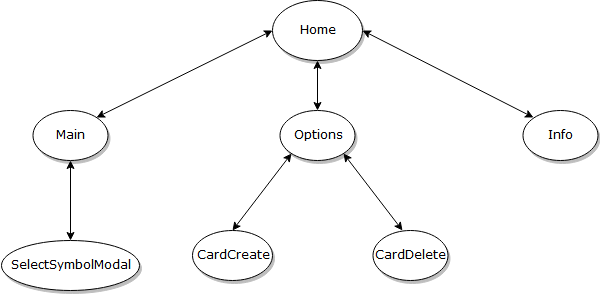
\includegraphics[height=7cm,keepaspectratio]{FreeAACViews}
  \caption[FreeAAC-sovelluksen näkymäpuu.]
  {FreeAAC-ohjelmiston näkymäpuu.}
  \label{fig:FreeAACViews}
\end{figure}

FreeAAC:n Ionic-näkymissä sisältö on jaettu kahden eri päätason HTML-elementin sisälle: \texttt{ion-header} ja \texttt{ion-content}. \texttt{Ion-header}-lohkossa sijaitsevat näkymän ylälaitaan tuleva teksti, joka kertoo missä näkymässä ollaan tällä hetkellä. Lisäksi lohkoon voidaan sijoittaa valikkotoimintoja. \texttt{Ion-content}-lohkossa sijaitsee näkymän varsinainen pääsisältö.

\texttt{Home}-näkymä on FreeAAC-ohjelmiston ensimmäinen näkymä ja se sisältää ohjelmiston päävalikon. Päävalikossa sijaitsevat painikkeet, joita klikkaamalla käyttäjä pääsee keskustelunäkymään (\texttt{Main}), asetusnäkymään (\texttt{Options}) tai infonäkymään (\texttt{Info}). \texttt{Home}-näkymän komponenttitiedostossa ei ole muita kuin näkymän vaihtamiseen liittyviä aliohjelmia.

\begin{figure}[h]\centering
  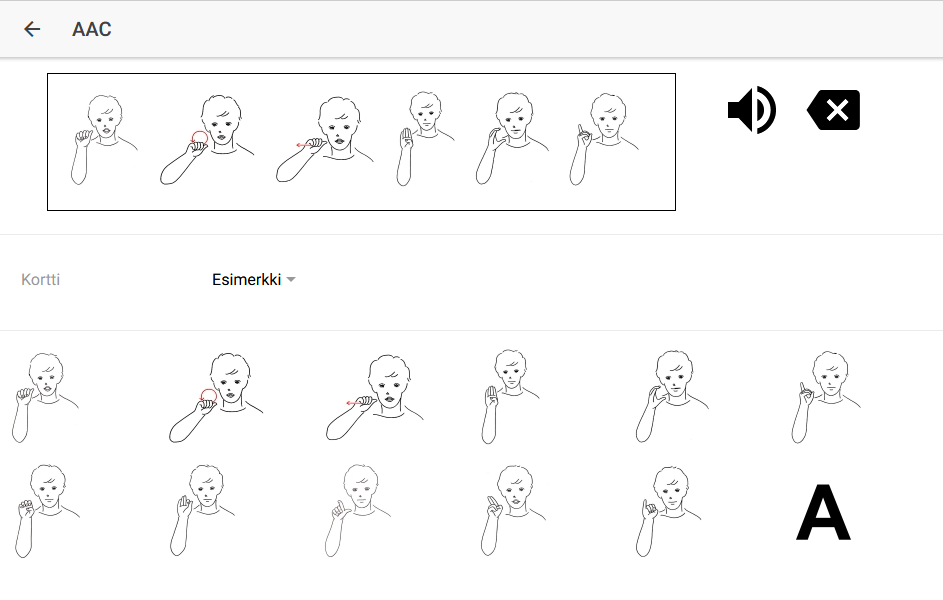
\includegraphics[height=10cm,keepaspectratio]{main-view-layout}
  \caption[FreeAAC-ohjelmiston kommunikointinäkymä.]
  {FreeAAC-ohjelmiston kommunikointinäkymä.}
  \label{fig:main-view-layout}
\end{figure}

\colorbox{YellowGreen}{// TODO: Yhteinäinen tapa käsitellä näkymien nimiä}

Ohjelmiston tärkein näkymä on kommunikointinäkymä eli \texttt{Main}-niminen näkymä, jossa sijaitsevat ohjelmiston varsinaiset kommunikointityökalut. \texttt{Main}-näkymä on kuvassa \ref{fig:main-view-layout}. \texttt{Main}-näkymän komponenttitiedosto sisältää viestilaatikon päivittämiseen sekä korttien tietojen lataamiseen tarvittavat aliohjelmat. Korttien lataamiseen käytetään \texttt{CardDataProvider}-luokkaa, joka on injektoitu mukaan komponenttiin sen konstruktorissa.

\texttt{Options}-näkymä on kokoomanäkymä ohjelmiston hallintaa varten. \texttt{Options}-näkymän kautta käyttäjä pääsee siirtymään korttien luontinäkymään (\texttt{CardCreate}) ja korttien poistonäkymään (\texttt{CardDelete}).

\begin{figure}[h]\centering
  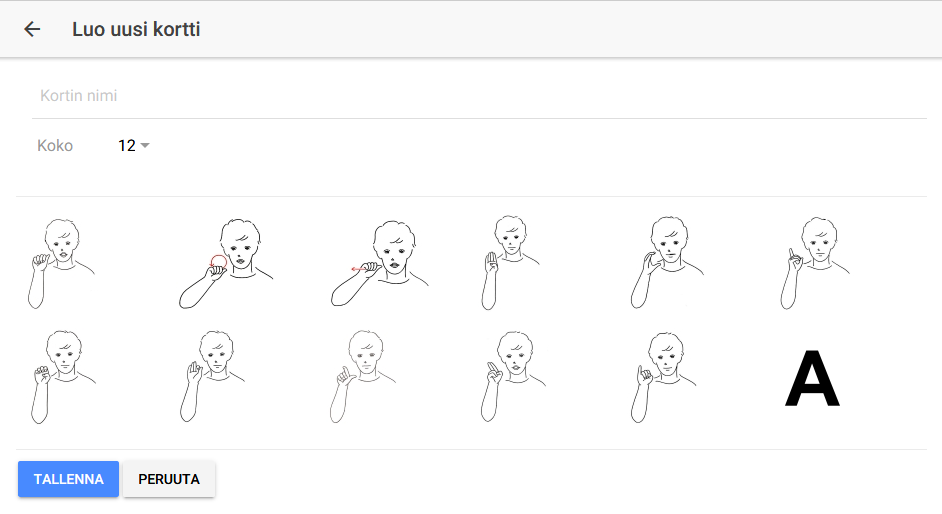
\includegraphics[height=9cm,keepaspectratio]{card-create-layout}
  \caption[FreeAAC-ohjelmiston korttien luontinäkymä.]
  {FreeAAC-ohjelmiston korttien luontinäkymä.}
  \label{fig:card-create-layout}
\end{figure}

Kortteja luodaan ohjelmiston \texttt{CardCreate}-näkymässä. \texttt{CardCreate}-näkymä on kuvassa \ref{fig:card-create-layout}. \texttt{CardCreate}-näkymässä kortille voidaan valita nimi, koko ja liittää siihen kuvia kuvakirjastosta. Kaikki edellä mainitut kentät ovat pakollisia ja käyttäjälle näytetään \texttt{toast}-virheilmoitus, jos jokin tieto puuttuu. \texttt{Toast}-virheilmoitukset käyttävät Ionicin \texttt{ToastController}-luokkaa. Kuvia valitaan erillisen ponnahdusikkunan kautta ja Ionic-sovelluksessa ponnahdusikkunoiden näyttämisestä vastaa \texttt{ModalController}-luokka. Korttien tallentaminen tapahtuu \texttt{CardDataProvider}-luokan kautta.

\begin{figure}[h]\centering
  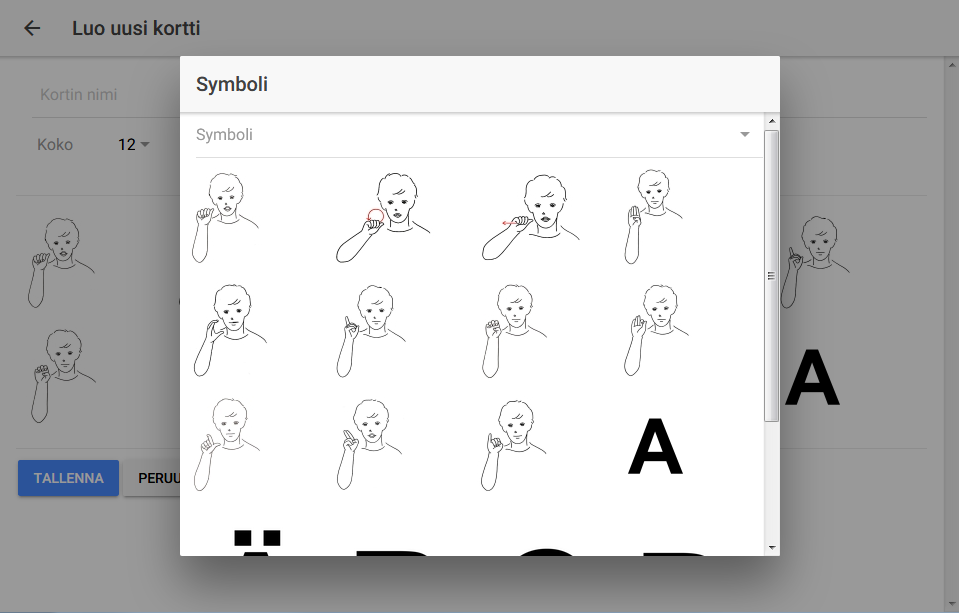
\includegraphics[height=10cm,keepaspectratio]{select-symbol-modal-layout}
  \caption[FreeAAC-ohjelmiston korttisymbolien valintanäkymä.]
  {FreeAAC-ohjelmiston korttisymbolien valintanäkymä.}
  \label{fig:select-symbol-modal-layout}
\end{figure}

Kuvien valintaa varten aukeava ponnahdusikkuna sisältää \texttt{SelectSymbolModal}-näkymän. \texttt{SelectSymbolModal}-näkymän sisältävä ponnahdusikkuna on kuvassa \ref{fig:select-symbol-modal-layout}. Näkymässä kuvan voi valita eri kategorioista. Kategoria valitaan pudotusvalikosta. \texttt{SelectSymbolModal}-näkymän komponenttitiedosto sisältää kuvan tallentamiseen ja ponnahdusikkunan sulkemiseen liittyvät aliohjelmat. FreeAAC-ohjelmiston kuvakirjasto koostuu Papunet-sivuston tarjoamasta Creative Commons -lisenssin alaisesta kuvapankista.

Kortteja voidaan poistaa erillisessä CardDelete-näkymässä. CardDelete-näkymä koostuu pudotusvalikosta, josta voidaan valita mikä kortti halutaan poistaa sekä vahvistuspainikkeesta. Korttilistaus ladataan \texttt{CardDataProvider}-luokan avulla ja myös poistokomento kulkee samaa reittiä pitkin.

Info-näkymässä listataan FreeAAC-sovellukseen liittyviä tietoja. Info-näkymä on staattinen eikä siinä ole toiminallisuuksia.

FreeAAC:lla on kaksi palveluluokkaa: \texttt{CardDataProvider} ja \texttt{ImageDataProvider}. \texttt{CardDataProvider}-olion tehtävä on tarjota näkymäkomponenteille tietoa olemassa olevista korteista. \texttt{ImageDataProvider}-olio huolehtii ohjelmiston kuvakirjaston eri kuvien toimittamisesta näkymäkomponenteille.

Ionic tarjoaa ohjelmistokehittäjän käyttöön \texttt{Ionic Storage} -nimisen tallennuspalvelun. \texttt{Ionic Storage} valitsee tallennustilan dynaamisesti ajoympäristöstä riippuen. Natiivissa kontekstissa \texttt{Ionic Storage} suosii \texttt{SQLite}-tietokantaa, kun taas WWW-sovelluksessa tai progressiivisena WWW-sovelluksessa ensisijainen tallennustila on \texttt{IndexedDB}-tietokanta. Jos \texttt{IndexedDB}:n käyttö ei jostain syystä ole mahdollista, yrittää \texttt{Ionic Storage} seuraavaksi käyttää \texttt{WebSQL}-tietokantaa tai selaimille varattua \texttt{Localstorage}-tallennustilaa.

\texttt{Ionic Storagen} monimutkaisuus ja dynaamisuus heijastelee hyvin progressiivisten WWW-sovellusten tallennusongelmia. Jokaisella edellä mainituista tallennusmahdollisuuksista on omat vahvuutensa ja heikkoutensa. Tämän takia tiedon tallentaminen massamuistiin jätettiin FreeAAC-ohjelmiston toteutuksen ulkopuolelle.

\section{Käytettävyysnäkökulma}

\colorbox{YellowGreen}{// TODO: Pura tämä luku ja liitä näkymistä kertovaan osuuteen ja arvioivaan osuuteen}

FreeAAC-ohjelmiston käytettävyysvaatimukset johdettiin yleisten suositusten perusteella sekä edellisissä kappaleissa mainittujen ominaisuuksien perusteella.

1. \textit{FreeAAC-ohjelmiston tulisi noudattaa yleisiä käytettävyysvaatimuksia, mutta myös sen lisäksi ottaa huomioon erityisryhmien, erityisesti autististen käyttäjien, käytettävyysvaatimukset huomioon.} \hyperref[general-usability-requirements]{(Luku 3.4.1, s. 15)}

2. \textit{FreeAAC-ohjelmiston värityksen tulisi olla pääväreihin perustuva, selkeä ja sen näkymissä tulisi olla riittävästi kontrastia.} \hyperref[AAC-colors]{(Luku 3.4.1, s. 17)}

3. \textit{Abstraktien symbolien käyttämistä tulisi välttää, sillä autistiset käyttäjät eivät välttämättä ymmärrä niiden merkitystä samalla tavalla kuin eritysryhmiin kuulumattomat käyttäjät.} \hyperref[AAC-abstract-symbols]{(Luku 3.4.1, s. 17)}

4. \textit{FreeAAC-ohjelmiston käytettävyyttä arkielämän nopeaa reagointia vaativissa tilanteissa lisäisi mahdollisimman perinpohjainen mahdollisuus räätälöintiin.} \hyperref[AAC-context-settings]{(Luku 3.4.1, s. 15)}

5. \textit{Käyttäjien mahdollisten motoristen haasteiden vuoksi näkymien tulisi olla pääosin staattisia ja niissä ei saisi olla nopeaa reagointia vaativia tapahtumia.} \hyperref[AAC-staticity]{(Luku 3.4.1, s. 15)}

FreeAAC-sovellus käyttää Ionicin oletuselementtejä ja oletusteemaa. Ionicin mukaan oletuselementit ja oletusteema noudattavat Applen iOS-designperiaatteita sekä Googlen Material Design -määrityksiä.  

Valikkonäkymien lisäksi käytettävyysratkaisuja on tehty erityisesti kommunikaationäkymässä (\texttt{Main}) ja korttien asetusnäkymissä (\texttt{CardCreate} ja \texttt{CardDelete}). Kommunikaationäkymä koostuu kolmesta eri komponentista: viestilaatikko, korttivalinta ja symbolivalinta. Viestilaatikkossa näkyvät käyttäjän valitsemat symbolit järjestyksessä. Käyttäjä voi poistaa symboleita yksi kerrallaan viimeisestä symbolista alkaen. Symbolikortti valitaan pudotusvalikosta, josta löytyvät käyttäjän kortinluonti-näkymässä tekemät kortit. Sivun alalaidassa näkyvät kortin symbolit, joista käyttäjä voi valita haluamansa symbolit viestilaatikkoon.

\chapter{Toteutuneen sovelluksen arviointi}

\colorbox{YellowGreen}{// TODO: Alusta tämä luku paremmin}

Rivimäärien käyttäminen ohjelmiston arviointiin ei ole täysin ongelmatonta, mutta eri tiedostojen rivimääriä analysoimalla voidaan saada perustason tietämystä ohjelmiston rakenteesta ja oleellisista osista. Edes ohjelmakoodin rivin määrite ei ole täysin yksiselitteinen asia, sillä yksi ohjelmakoodin looginen osa voidaan rivittää eri ohjelmointiperiaatteiden perusteella useille riveille. Lisäksi ohjelmakoodin rivimäärään vaikuttavat muutkin luettavuusmääritteet kuten tyhjien rivien käyttö sekä kommenttien määrä. FreeAAC-ohjelmiston rivien kokonaismäärä laskettiin ilman tyhjien tai kommenttirivien vähentämistä kokonaismäärästä.

Suurin osa riveistä sijaitsee ohjelmistokehittäjän itse laatimissa mallitiedostoissa ja näitä hallinnoivissa komponenttitiedostoissa. Näissä tiedostoissa olevien rivien määrä on 783. Jos 7528 riviä sisältävä \texttt{package-lock.json}-tiedosto otetaan pois laskuista, on ohjelmiston kokonaisrivimäärä 1320 ja ohjelmistokehittäjän pääasiallisesti tuottamat tiedostot sisältävät noin 59,32\% ohjelmiston kokonaisrivimäärästä.

Koska rivimäärien laskeminen ei anna kovin hyvää kuvaa ohjelmistosta, on ohjelmistojen analysoimiseen kehitetty edistyneempiä menetelmiä. Halsteadin monimutkaisuusmetriikat ovat tapoja mitata ohjelman ominaisuuksia. Maurice Howard Halstead pyrki niiden avulla muodostamaan tavan mitata ohjelman ominaisuuksia vertailukelpoisesti. Halsteadin monimutkaisuusmetriikoiden muodostamista varten tarvitaan neljä perusmuuttujaa: uniikkien operaattorien määrä ($n_1$), uniikkien operandien määrä ($n_2$), operaattorien kokonaismäärä ($N_1$) ja operandien kokonaismäärä ($N_2$).

Näiden neljän perusmuuttujan pohjalta voidaan johtaa useita eri monimutkaisuusmetriikoita:

\begin{center}
    \begin{tabular}{ | l | l | l |}
    \hline
    \textbf{Metriikka} & \textbf{Merkitys} & \textbf{Kaava} \\ \hline
    $n$ & Sanasto & $n_1 + n_2$ \\ \hline
    $N$ & Koko & $N_1 + N_2$ \\ \hline
    $V$ & Määrä & $N * log2 n$ \\ \hline
    $D$ & Haastavuus & $n1/2 + N_2/n_2$ \\ \hline
    $E$ & Työmäärä & $V * D$ \\ \hline
    $B$ & Virheet & $V / 3000$ \\ \hline
    $T$ & Testausaika & $E / k$ \\ \hline
    \end{tabular}
\end{center}

Perusmuuttujien arvot FreeAAC-ohjelmistolle:

\begin{center}
    \begin{tabular}{| l | l | l | l | l |}
    \hline
    \textbf{Tiedosto} & \textbf{$n_1$} & \textbf{$n_2$} & \textbf{$N_1$} & \textbf{$N_2$} \\ \hline
    MainPage & 65 & 55 & 213 & 92 \\ \hline
    CardCreatePage & 62 & 53 & 192 & 88 \\ \hline
    SelectSymbolModalPage & 27 & 20 & 50 & 22 \\ \hline
    HomePage & 26 & 16 & 56 & 31 \\ \hline
    OptionsPage & 24 & 16 & 39 & 14 \\ \hline
    CardDataProvider & 23 & 15 & 55 & 63 \\ \hline
    ImageDataProvider & 22 & 14 & 52 & 16 \\ \hline
    CardDeletePage & 21 & 17 & 42 & 20 \\ \hline
    Card & 17 & 22 & 55 & 63 \\ \hline
    WordSymbol & 16 & 14 & 47 & 16 \\ \hline
    InfoPage & 13 & 10 & 26 & 10 \\ \hline
    \end{tabular}
\end{center}

Monimutkaisuusmetriikoiden arvot FreeAAC-ohjelmistolle:

\begin{center}
    \begin{tabular}{| l | l | l | l | l | l | l | l |}
    \hline
    \textbf{Tiedosto} & \textbf{$n$} & \textbf{$N$} & \textbf{$V$} & \textbf{$D$} & \textbf{$E$} & \textbf{$B$} & \textbf{$T$} \\ \hline
    MainPage & 120 & 305 & 1471.17... & 54.36... & 79978.03... & 0.49... & ~4443s  \\ \hline
    CardCreatePage & 115 & 280 & 1314.33... & 51.47... & 67651.01... & 0.44... & ~3758s \\ \hline
    SelectSymbolModalPage & 47 & 72 & 277.73... & 14.85... & 4124.28... & 0.09... & ~229s \\ \hline
    HomePage & 42 & 87 & 301.97... & 25.19... & 7605.86... & 0.10 & ~423s \\ \hline
    Card & 39 & 118 & 290.70... & 24.34... & 7075.83... & 0.10... & ~393s  \\ \hline
    CardDeletePage & 38 & 62 & 220.41... & 12.35... & 2722.75... & 0.07... & ~151s   \\ \hline
    OptionsPage & 38 & 62 & 220.41... & 12.35... & 2722.75... & 0.07... & ~151s  \\ \hline
    CardDataProvider & 38 & 118 & 288.64... & 48.30... & 13941.12... & 0.10... & ~775s  \\ \hline
    ImageDataProvider & 36 & 68 & 268.84... & 12.57... & 3379.65... & 0.09... & ~188s \\ \hline
    WordSymbol & 30 & 63 & 230.62... & 9.14... & 2108.56... & 0.08... & ~117s  \\ \hline
    InfoPage & 23 & 36 & 117.61... & 6.50... & 764.48... & 0.04... & ~42s  \\ \hline
    \end{tabular}
\end{center}

Sanastometriikan (n) perusteella FreeAAC-ohjelmiston kaksi sanastoltaan selkeästi laajinta tiedostoa ovat \texttt{MainPage} ja \texttt{CardCreatePage}. Muut tiedostot ovat laajuudeltaan suunnilleen samankokoisia keskenään. Ainoastaan InfoPage-tiedosto on selkeästi muita pienempi.

Kokometriikka (N) noudattaa pitkälti samoja linjoja, mutta \texttt{Card}- ja \texttt{CardDataProvider}-tiedostojen koko on suhteellisesti suurempi sanastometriikkaan verrattuna kuin muiden tiedostojen. Tämä kertoo näissä tiedostoissa olevien luokkien muista suuremmasta toisteisuudesta. Ne sisältävät useita pieniä metodeja, jotka ovat kytkeytyneet korttien käsittelyyn ja yksittäisen kortin tietojen tarjoamiseen muille luokille.

Testausyritys Verifysoftin mukaan (lainaus) tiedoston määrämetriikan (V) tulisi olla vähintään 100 ja korkeintaan 8000. Kaikki FreeAAC-ohjelmiston tiedostot pysyvät näiden rajojen sisällä. Tiedostojen keskinäisissä määrämetriikoissa ei ole mitään edellisistä metriikoista poikkeavaa.

Haastavuusmetriikka (D) pyrkii mittaamaan tiedoston virhealttiutta. Laajimpien \texttt{MainPage}- ja \texttt{CardCreatePage}-tiedostojen lisäksi korkea haastavuusmetriikka on myös \texttt{CardDataProvider}-tiedostolla.
\colorbox{YellowGreen}{// TODO: Lihota}

Tiedostojen työmäärät (E) noudattavat samoja linjoja kuin haastavuusmetriikka. Vaikka \texttt{CardDataProvider} ei ole sanastoltaan tai kooltaan yhtä suuri kuin kaksi suurinta tiedostoa, sisältää se kuitenkin sellaisia rakenteita, jotka nostavat sen kuitenkin yhtä merkittäväksi osaksi ohjelmaa.

Virhemetriikka (B) on arvio tiedostossa esiintyvien ohjelmistovirheiden määrästä. Verifysoftin mukaan tiedoston virhemetriikan arvon tulisi olla alle 2. Jokainen FreeAAC-ohjelmiston tiedosto alittaa tämän arvon.

Viimeinen tässä pro gradu -työssä tarkasteltava metriikka on testausaika (T). Sillä pyritään arvioimaan tiedostoon testaamisen kuluvaa aikaa sekunneissa. Testausaikametriikka tuottaa muiden metriikoiden mukaisia arvoja. Testausajan laskemiseen käytetään arvoa \textit{k}, joka määrittyy monen tekijän perusteella. Arvoon vaikuttavat asiat kuten testaajien kokemus ja tiedoston kriittisyys ohjelman toimivuuden kannalta, joten tämän pro gradu -työn puitteissa testausaikametriikasta ei juurikaan saada lisäarvoa FreeAAC-ohjelmiston arviointiin.

FreeAAC-ohjelmisto ei ylitä Halsteadin monimutkaisuusmetriikoiden ohjearvoja ja eri tiedostojen arvot eri metriikoiden kohdalla ovat johdonmukaisia keskenään. FreeAAC-ohjelmisto täten noudattaa Halsteadin monimutkaisuusmetriikoiden perusteella hyvän ja ehjän ohjelmiston rakennetta. Halsteadin monimutkaisuusmetriikoiden todistusvoima ei kuitenkaan ole aukoton ja parempia tuloksia saataisiin aikaan vertaamalla FreeAAC-ohjelmiston monimutkaisuusmetriikoiden arvoja muiden vastaavien ohjelmistojen arvoihin. 

Vertaileva tutkimus muihin avusteisen kommunikaation sovelluksiin on kuitenkin rajattu tämän pro gradu -työn ulkopuolelle, sillä suurin osa avusteisen kommunikaation sovelluksista on kehitetty kaupalliseen käyttöön ja avoimen lähdekoodin sovelluksia ei juurikaan ole tarjolla.
\colorbox{YellowGreen}{// TODO: prototyyppiohjelmisto jne.}

\begin{figure}[h]\centering
  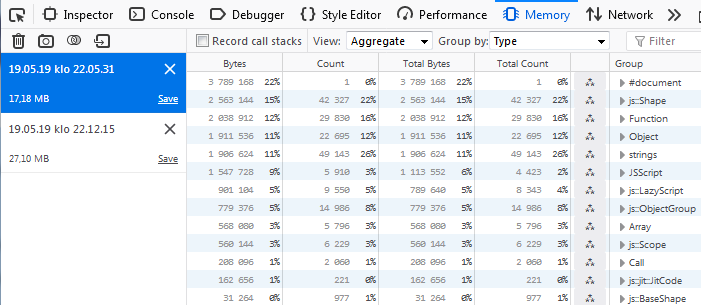
\includegraphics[height=6cm,keepaspectratio]{memory-use-idle}
  \caption[FreeAAC-sovelluksen muistinkäyttö lepotilassa.]
  {FreeAAC-sovelluksen muistinkäyttö lepotilassa.}
  \label{fig:memory-use-idle}
\end{figure}

\begin{figure}[h]\centering
  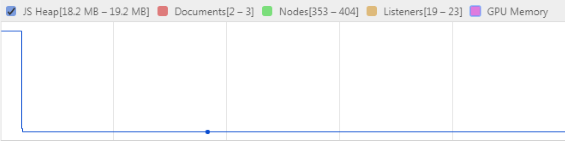
\includegraphics[height=4cm,keepaspectratio]{chromium-memory-use-idle}
  \caption[FreeAAC-sovelluksen muistinkäyttö lepotilassa graafina.]
  {FreeAAC-sovelluksen muistinkäyttö lepotilassa.}
  \label{fig:chromium-memory-use-idle}
\end{figure}

\begin{figure}[h]\centering
  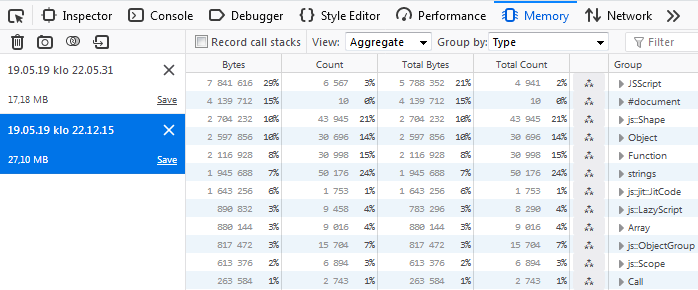
\includegraphics[height=6cm,keepaspectratio]{memory-use-stress}
  \caption[FreeAAC-sovelluksen muistinkäyttö käytön aikana.]
  {FreeAAC-sovelluksen muistinkäyttö käytön aikana.}
  \label{fig:memory-use-stress}
\end{figure}

\begin{figure}[h]\centering
  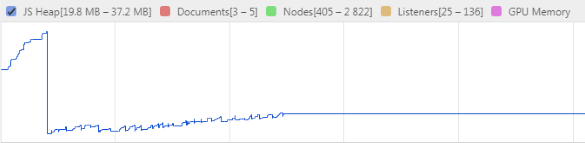
\includegraphics[height=4cm,keepaspectratio]{chromium-memory-use-stress}
  \caption[FreeAAC-sovelluksen muistinkäyttö käytön aikana graafina.]
  {FreeAAC-sovelluksen muistinkäyttö käytön aikana.}
  \label{fig:chromium-memory-use-stress}
\end{figure}

Progressiivisten WWW-sovellusten muistinkäyttöä arvioitiin kappaleessa 3.2. FreeAAC-ohjelmiston muistinkäyttöä mitattiin Firefox-selaimen kehitystyökaluilla ottamalla mittauksia sekä ohjelman alkutilassa \ref{fig:memory-use-idle} sekä käytön aikana \ref{fig:memory-use-stress}. Lisäksi muistinkäyttöä seurattiin samalla tavoin Chromium-selaimen kehitystyökaluilla ohjelman alkutilassa \ref{fig:chromium-memory-use-idle} sekä käytön aikana \ref{fig:chromium-memory-use-stress}. 

Korkein mitattu muistinkäyttö rasitukseessa oli 37MB. Liitteissä C ja D on listattu joukko yleisten tablettitietokoneiden ja matkapuhelinten muistinkäyttörajoja ohjelmistoille. Ainoat listatut laitteet, joiden muistinkäyttörajan FreeAAC-ohjelmisto ylittää ovat HTC:n valmistamia matkapuhelimia vuosilta 2010 ja 2011. Muistinkäyttö nousee prosentuaalisesti varsin ison määrän käytön aikana, mutta kokonaismäärä ei aiheuta ongelmia millekään nykyaikaiselle mobiililaitteelle.

Muistinkäyttökäyriä tutkimalla nähdään, että ohjelman käynnistyessä muistinkäyttö nousee hetkellisesti, mutta ensimmäisen roskienkeruun jälkeen muistinkäyttö putoaa heti käynnistyksen jälkeistä tilannetta huomattavasti matalammaksi. Näin käy sekä ilman käyttäjän syötettä, että aktiivisen käytön aikana. Ilman käyttäjän syötteitä FreeAAC-ohjelmiston muistinkäyttö ei nouse ollenkaan. Ohjelmistossa ei ole toimintoja, jotka käyttäisivät muistia silloin kun käyttäjä ei aktiivisesti käytä ohjelmistoa. Tämä on tärkeää, sillä avusteisen kommunikaation sovellusta käytetään useasti vain hetkellisesti. Käytön aikana muistinkäyttö nousee hitaasti ja 5 minuutin testikäytön aikana ei saatu aikaan suuria hyppäyksiä ylöspäin. FreeAAC-ohjelmiston muistinkäyttö vaikuttaa tasaiselta.

FreeAAC-ohjelmiston ohjelmakoodin määrä on maltillinen verrattuna ominaisuusvaatimuksiin, mikä parantaa ohjelmiston ylläpidettävyyttä ja testattavuutta. Ohjelmistossa on myös hyvin vähän sisäisiä riippuvuuksia, koska Angular-ohjelmistokehyksen sekä TypeScript-ohjelmointikielen avulla ohjelmistosta saatiin helposti tehtyä modulaarinen.
\colorbox{YellowGreen}{// TODO: Lähde?}

Näkymien HTML-formaatti ei juurikaan aiheuttanut ohjelmistoteknisiä haasteita tai käytettävyysongelmia. Ainoastaan symbolien vapaa asemointi kortilla osoittautui sen verran haastavaksi tehtäväksi, että sitä ei toteutettu. HTML-kieli on alunperin tarkoitettu dokumenttien hierarkkiseksi ja rakenteelliseksi kuvauskieleksi, joten HTML-elementtien kelluvaa asemointia toisiinsa nähden ei ole helpoin toteuttaa sen avulla. Kelluvien elementtien toteuttaminen on kyllä mahdollista oikeanlaisten CSS-määritysten avulla, mutta tämä vaatisi erillisen asemointipalvelun rakentamista ohjelmistoon sekä CSS-luokkien lisäilyä ja poistamista reaaliajassa. Perinteisessä mobiilisovelluksessa elementtien vapaa asemointi olisi todennäköisesti helpompaa.
\colorbox{YellowGreen}{// TODO: Lähteitä ja muista lisätä ominaisuusvaatimuksiin!}

Kenties haastavin osuus FreeAAC-ohjelmiston toteuttamisessa oli tietojen tallentaminen. Kuten luvussa 4.3 todettiin, progressiivisille WWW-sovelluksille ei ole luontevaa tallennustilaa, sillä selainten oikeuksien määrä on hyvin tarkasti rajoitettua tietoturvasyistä. Kuvat voidaan liittää mukaan sovellukseen, mutta korttien asetuksien tallentaminen ei ole yksinkertaista. Natiivisovelluksilla on suora pääsy rajattuun massamuistitilaan, mutta WWW-sovelluksissa tiedot tulee tallentaa muualle. Täten massamuistiin liittyvät operaatiot jätettiin tämän pro gradu -työn ulkopuolelle.
\colorbox{YellowGreen}{// TODO: Korjaa hieman aiempaa kerrottua vastaavaksi.}

\section{Käytettävyysnäkökulma}

Käytettävyyden perusvaatimusten osalta FreeAAC-ohjelmiston toteutuksessa ei ilmennyt suuria haasteita. Ionicin tarjoama oletusteema on tehty yleisten käytettävyysvaatimusten mukaisesti käyttämällä erityisesti Googlen ja Applen mobiilikäyttöjärjestelmien käytettävyysohjeita, joten suurin osa ohjelmistosta pystyy käyttämään sitä suoraan ilman muutoksia. Tämä nopeuttaa ohjelmiston kehittämistä ja parantaa ohjelmiston ulkoasun käytettävyyttä sekä yhtenäisyyttä.

FreeAAC-sovelluksen elementit ovat riittävän isoja, jotta niiden valitseminen ja toiminnallisuuksien ymmärtäminen on helpompaa kun ohjelmistoa ajetaan pieninäyttöisillä mobiililaitteilla. \colorbox{YellowGreen}{// TODO: Lähde käytettävyysohjeista?} Suuret elementit myös rajoittavat yhteen näkymään mahtuvien ominaisuuksien määrää, mikä auttaa pitämään näkymät riittävän yksinkertaisina käyttäjälle.

FreeAAC-ohjelmiston opittavuutta helpottaa se, että näkymät muistuttavat paljolti toisiaan. FreeAAC-ohjelmistossa ei ole moodeja eikä samoja toimintoja voi suorittaa usealla eri tavalla. Tämä lisää sekä opittavuutta, että muistettavuutta. 

Tehokkuus on määre, jota parhaiten voidaan mitata suorittamalla käyttäjätutkimus, jossa käyttäjälle annettuun tehtävään käytettyä aikaa sekä siinä ilmenneitä haasteita pyritään mittaamaan. Koska tutkielmassa ei suoritettu käyttäjätutkimusta vaan suunnittelutieteellinen tutkimus, on tehokkuutta tutkittava muiden keinojen avulla. Yksi tapa arvioida tehokkuutta on muodostaa lista yleisimpiin toimintoihin vaadittavien välivaiheiden määristä ja arvioida tehokkuutta niiden perusteella.

\begin{center}
    \begin{tabular}{| l | l |}
    \hline
    \textbf{Toiminto} & \textbf{Välivaiheiden määrä} \\ \hline
    Kommunikointinäkymään siirtyminen & 1  \\ \hline
    Viestin kirjoittaminen & 3 + (x * symbolien määrä)\\ \hline
    Kortin luonti & 5 + (x * symbolien määrä) \\ \hline
    Kortin poisto & 3  \\ \hline
    \end{tabular}
\end{center}

Välivaiheiden määrästä ei voi suoraan muodostaa täyttä kuvaa ohjelmiston tehokkuudesta tai muista laadullisista tekijöistä, mutta niitä voidaan verrata psykologisiin tutkimuksiin ihmisten lyhytkestoisesta muistista. Yksi kaikkien aikojen eniten lainatuista psykologian tutkimuksista \parencite[]{most-quoted-psych} on George A. Millerin \textit{The Magical Number Seven, Plus or Minus Two} \parencite[]{magical-number-seven}, jonka keskeiset havannot liittyvät ihmisen kykyyn muistaa tiettyjä määriä perusalkioita kerrallaan.

Millerin mukaan ihminen pystyy muistamaan $7 \pm 2$ perusalkiota lyhytkestoista muistia käyttämällä. Lisäksi Millerin mukaan ihminen käsittelee näitä alkiota kahden tai kolmen alkion ryppäissä. Yksikään FreeAAC-ohjelmiston perustoiminto ei ylitä tätä Millerin laiksikin kutsuttua perusoletusta. Täten FreeAAC-ohjelmiston perustoimintojen käyttö on ainakin teoreettisella tasolla ihmisen lyhytkestoisen muistin rajojen sisällä. Tämä parantaa ohjelmiston tehokkuutta, muistettavuutta ja vähentää käyttäjän tekemien virheiden määrää.

FreeAAC-ohjelmiston virhealttiutta vähentää myös se, että käyttäjän syötemahdollisuuksia on rajattu. Käyttäjä ei yleensä voi päätyä tilanteisiin, jossa tapahtuu jotain peruuttamatonta. Ainoastaan symbolin poistaminen kortilta tai kortin poistaminen kokonaisuudessaan voi aiheuttaa käyttäjälle tilanteen, jossa menetetään paljon tehtyä työtä. Nämä ominaisuudet on kuitenkin piilotettu erilliseen salasanasuojattuun näkymään, joten riski peruuttamattomaan virheeseen on minimoitu.

Tyydyttävyyttä on hankala mitata ilman koekäyttäjiä, mutta yleisten laatutekijöiden arviointi ja huomioon ottaminen ohjelmiston toteutuksessa lisää tyydyttävyyttä. Voidaan esimerkiksi olettaa, että ohjelmiston yhtenäinen ulkoasu lisää opittavuuden ja tehokkuuden lisäksi myös tyydyttävyyttä.

FreeAAC-ohjelmistolle listattiin myös joukko erityisryhmien käytettävyysvaatimuksia. Etenkin autististen käyttäjien tarpeet pyrittiin ottamaan huomioon.

Sovelluksen käyttämiseen ei tarvita eritysryhmille mahdollisesti motorisesti haastavia eleitä kuten pyyhkäisyjä. Erityisesti autisteilla on usein ongelmia hienomotoristen liikkeiden suorittamisessa, vaikka autististen käyttäjien yksilökohtaiset erot ovat tässäkin suuria \parencite[]{motor-skills-autism}.

FreeAAC-ohjelmiston valikot on toteutettu perinteisellä tavalla painikkeita hyödyntämällä. Monessa mobiilisovelluksessa navigointi tapahtuu niin sanotun \textit{hampurilaisvalikon} avulla, mutta autistisille käyttäjille tarkoitetussa ohjelmistossa abstraktien symbolien käyttö voi olla ongelmallista (lähde), joten ohjelmistossa ei käytetä tätä yleistä ratkaisua.

FreeAAC:n ulkoasusta tehtiin mustavalkoinen, jotta symbolit ja käyttäjän mahdollisesti ottamat kuvat erottuvat paremmin muista elementeistä.

FreeAAC-ohjelmiston näkymissä ei ole toimintoja tai elementtejä, joiden käyttäminen vaatii nopeaa reagointia. Näkymistä on pyritty rakentamaan mahdollisimman yksinkertaisia ja tämän esimerkiksi korttien luontinäkymä ja korttien poistonäkymä on erotettu toisistaan.

\colorbox{YellowGreen}{// TODO: korttien vaihtaminen ja korttien koko}

\chapter{Pohdinta}

Pro gradu -työn tärkein tulos oli se, että olemassa olevan tutkimuksen pohjalta luotujen vaatimusten noudattaminen ei tuottanut ongelmia. Progressiiviset WWW-sovellukset, ja tarkemmin rajattuna Ionic-kehys, sopii avusteisen kommunikaation sovelluksen kehittämiseen sekä ohjelmistoteknisestä, että käytettävyysnäkökulmasta. Lisäksi saatiin kattavasti tietoa siitä, mitä laatutekijöitä avusteisen kommunikaation ohjelmiston kehittämiseen liittyy.

Suunnittelutieteellisen tutkimuksen käyttäminen progressiivisten WWW-sovellusten ohjelmistoteknisen puolen tutkimiseen oli toimiva tapa saada aikaan perustietoa tutkimuksessa esitetyn käyttötapauksen vaatimuksista ja niiden toteuttamisen haasteista. Progressiiviset WWW-sovellukset ovat edelleen niin tuore ilmiö, että olemassa olevaa tutkimusta oli haastavaa löytää. Tämän takia artefaktin kehittäminen oli tärkeää, sillä sen avulla saatiin paljon ensikäden perustietoa progressiivisten WWW-sovellusten toiminnasta ilman nojaamista olemassa olevaan tutkimukseen.

Käytettävyystutkimuksen näkökulmasta suunnittelutieteellisen tutkimusmetodin käyttäminen oli haastavampaa. Oli tärkeää ottaa huomioon käytettävyystekijät artefaktin suunnitteluvaiheessa, mutta varmempien johtopäätösten vetäminen valmiista artefaktista olisi kenties vaatinut käyttäjätutkimuksen tekemistä. Tästä syystä valmiin artefaktin tutkiminen käytettävyysnäkökulmasta jäi ehkä hieman pintapuoliseksi.

Pro gradu -työn vertaaminen olemassa olevaan tutkimukseen on haastavaa myös siitä syystä, että hyvin harva avusteista kommunikaatiota tutkivista tutkimusta lähestyi asiaa tietoteknisestä näkökulmasta. Ainoa selkeästi olemassa olevaa avusteisen kommunikaation ohjelmistoa tutkinut tutkimus, joka tämän pro gradu -työn aineistonkeruussa onnistuttiin löytämään, oli Comunicador-nimistä espanjankielisille käyttäjille suunnattua ohjelmistoa tutkinut tutkimus, jonka tuloksia käsiteltiin luvussa 3.4.1.

\colorbox{YellowGreen}{-- Pohdintaluvussa harjoitetaan itsenäistä ajattelua. Sen voi periaatteessa kirjoittaa ilman lähdekirjallisuutta, sillä tarkastelun kohteena on aiemmin kirjoitettamasi materiaali. Nyt tutkimuksen tuloksia on aika arvioida kriittisesti. Niitä verrataan aiempaan tutkimukseen ja pohditaan, mitä uutta tutkimus paljastaa aiheesta ja miten tulokset suhteutuvat aiempaan tutkimukseen – tukevatko vai ovatko ristiriidassa? Jos analyysivaiheessa on ollut vaikeuksia, niitä ei pidä lakaista maton alle; niiden puntaroiminen kertoo tutkimuksen läpinäkyvyydestä ja tulosten luotettavuudesta. --}

\chapter{Yhteenveto}

FreeAAC-ohjelmiston prototyyppi sisältää suurimman osan tarpeellisista ominaisuuksista ja siitä pystyttiin toteuttamaan toimiva sekä mahdolliseen koekäyttöön sopiva versio tutkielman aikarajoitteiden puitteissa. Tämän perusteella voidaan todeta, että ainakin perustasolla progressiiviset WWW-sovellukset vaikuttavat lupaavalta ja riittävän kypsältä teknologialta yksinkertaisten mobiilisovellusten toteuttamiseen.

Tämän pro gradu -työn pohjalta syntyi useita mahdollisia jatkotutkimuksen aiheita. Yksi FreeAAC-ohjelmiston toteutuksen ulkopuolelle jäänyt perusominaisuus oli massamuistitilan käyttö käyttäjän asetusten ja luotujen korttien pysyvään tallennukseen. Tämän ominaisuuden karsimista perusteltiin Ionic-ohjelmistokehyksen massamuistitallennuksen monimutkaisuudella ja vaihtoehtojen paljoudella. Voisi siis olla kannattavaa tutkia progressiivisten WWW-sovellusten massamuistitallennusvaihtoehtojen hyviä ja huonoja puolia erilaisissa tilanteissa.

Toinen tutkimuksen aikana esiin noussut puute oli eri erikoisryhmien parissa tehtyjen käytettävyystutkimuksien vähyys. Erityisesti modernien mobiililaitteiden ja kosketusnäyttöjen käytettävyyttä ei ole juurikaan ehditty tutkimaan näiden erityisryhmien näkökulmasta. Esimerkiksi käytettävyyden laatutekijöitä arvioidessa jouduttiin käyttämään yleisiä laatutekijöitä. Ei tiedetä esimerkiksi miten autismi vaikuttaa eri laatutekijöiden arviointiin.

Progressiivisten WWW-sovellusten muistinkäyttö oli yksi tässä tutkimuksessa tarkasteltu asia. Muistinkäyttö ei osoittautunut ongelmaksi tässä nimenomaisessa käyttötapauksessa, mutta tutkimuksen aihepiiriin ei kuulunut suuria määriä muistia vaativien progressiivisten WWW-sovellusten tutkiminen. FreeAAC-ohjelmiston toiminnallisuudet eivät vaadi suuria määriä laskentatehoa tai massiivisia muistiallokaatioita, joten täyttä kuvaa Ionic-ohjelmistokehyksen tai progressiivisten WWW-sovellusten suorituskyvystä ei saatu.

Yleisesti ottaen oli yllättävää miten pieni määrä ongelmia FreeAAC-ohjelmiston kehitystyössä ilmeni ja miten helposti suurin osa laadullisista vaatimuksista täyttyi. FreeAAC-ohjelmiston kehittämistä on tarkoitus jatkaa myös tämän pro gradu -työn jälkeen ja toivottavasti jonain päivänä ohjelmistosta on iloa muussakin kuin tutkimuskohteena.

%\printbibliography{gradubibtex}

\printbibliography

%\bibliography{gradubibtex}{}
%\bibliographystyle{plain}

\appendix

\section{FreeAAC-ohjelmiston ominaisuusvaatimukset}

Lähdemateriaalista johdetut ominaisuusvaatimukset FreeAAC-ohjelmistolle:

\begin{center}
    \begin{tabular}{ | l | l |}
    \hline
    \textbf{Ominaisuus} & \textbf{Toteutettu} \\ \hline
    Kommunikaatiokortit. & Kyllä \\ \hline
    Kuvien ja symbolien valitseminen kortilta viestiin. & Kyllä \\ \hline
    Viestin äänisynteesi. & Ei \\ \hline
    Korttien luominen ja poistaminen. & Kyllä \\ \hline
    Korttien koon määrittäminen. & Kyllä \\ \hline
    Kortin vaihtaminen. & Kyllä \\ \hline
    Kuvien valitseminen korteille valmiista kirjastosta. & Kyllä \\ \hline
    Kuvien valitseminen korteille kuvia ottamalla. & Ei \\ \hline
    Hallintapaneeli. & Kyllä \\ \hline
    Lukitusominaisuus hallintapaneeliin. & Ei \\ \hline
    Korttien ja asetusten tallentaminen laitteen massamuistiin. & Ei \\ \hline
    \end{tabular}
\end{center}

\section{FreeAAC-ohjelmiston tiedostot rivimäärittäin}

\begin{center}
    \begin{tabular}{ | l | l |}
    \hline
    \textbf{Tiedosto} & \textbf{Rivien lukumäärä} \\ \hline
    package-lock.json & 7528 \\ \hline
    cardcreate.ts & 112 \\ \hline
    variables.scss & 88 \\ \hline
    config.xml & 86 \\ \hline
    app.module.ts & 73 \\ \hline
    package.json & 66 \\ \hline
    image-data.ts & 53 \\ \hline
    main.ts & 52 \\ \hline
    index.html & 50 \\ \hline
    main.html & 41 \\ \hline
    cardcreate.html & 40 \\ \hline
    card.ts & 39 \\ \hline
    .gitignore & 36 \\ \hline
    app.component.ts & 36 \\ \hline
    card-data.ts & 36 \\ \hline
    app.scss & 32 \\ \hline
    selectsymbolmodal.ts & 32 \\ \hline
    service-worker.js & 31 \\ \hline
    home.ts & 29 \\ \hline
    carddelete.ts & 28 \\ \hline
    selectsymbolmodal.html & 28 \\ \hline
    tsconfig.json & 28 \\ \hline
    options.ts & 27 \\ \hline
    wordsymbol.ts & 26 \\ \hline
    options.html & 21 \\ \hline
    \end{tabular}
\end{center}

\begin{center}
    \begin{tabular}{ | l | l |}
    \hline
    \textbf{Tiedosto} & \textbf{Rivien lukumäärä} \\ \hline
    info.html & 20 \\ \hline
    home.html & 19 \\ \hline
    app.html & 18 \\ \hline
    .editorconfig & 16 \\ \hline
    info.ts & 14 \\ \hline
    cardcreate.module.ts & 13 \\ \hline
    carddelete.html & 13 \\ \hline
    carddelete.module.ts & 13 \\ \hline
    info.module.ts & 13 \\ \hline
    options.module.ts & 13 \\ \hline
    selectsymbolmodal.module.ts & 13 \\ \hline
    manifest.json & 12 \\ \hline
    tslint.json & 13 \\ \hline
    README.md & 8 \\ \hline
    ionic.config.json & 8 \\ \hline
    main.ts & 8 \\ \hline
    cardcreate.scss & 3 \\ \hline
    carddelete.scss & 3 \\ \hline
    home.scss & 3 \\ \hline
    info.scss & 3 \\ \hline
    options.scss & 3 \\ \hline
    selectsymbolmodal.scss & 3 \\ \hline
    main.scss & 0 \\ \hline
    \textbf{Yhteensä} & 8848 \\
    \hline
    \end{tabular}
\end{center}

\section{Muistinkäyttörajat yksittäiselle ohjelmistolle iOS-laitteissa}

Tablettitietokoneet lihavoitu.

\begin{center}
    \begin{tabular}{| l | l |}
    \hline
    \textbf{Malli} & \textbf{Muistinkäyttöraja} \\ \hline
    \textbf{iPad1} & 127MB  \\ \hline
    \textbf{iPad2} & 275MB \\ \hline
    \textbf{iPad3} & 645MB \\ \hline
    \textbf{iPad4} & 585MB \\ \hline
    \textbf{iPad Mini} & 297MB \\ \hline
    \textbf{iPad Mini retina} & 696MB \\ \hline
    \textbf{iPad Air} & 697MB \\ \hline
    \textbf{iPad Air 2} & 1383MB \\ \hline
    \textbf{iPad Pro 9.7"} & 1395MB  \\ \hline
    \textbf{iPad Pro 10.5”} & 3057MB \\ \hline
    \textbf{iPad Pro 12.9” (2015)} & 3058MB \\ \hline
    \textbf{iPad Pro 12.9” (2017)} & 3057MB \\ \hline
    \textbf{iPad Pro 11.0” (2018)} & 2858MB \\ \hline
    \textbf{iPad Pro 12.9” (2018)} & 4598MB \\ \hline
    iPhone4 & 325MB \\ \hline
    iPhone4s & 286MB \\ \hline
    iPhone5 & 645MB \\ \hline
    iPhone5s & 646MB \\ \hline
    iPhone6 & 645MB \\ \hline
    iPhone6+ & 645MB \\ \hline
    iPhone6s & 1396MB \\ \hline
    iPhone6s+ & 1392MB \\ \hline
    iPhoneSE & 1395MB \\ \hline
    iPhone7 & 1395MB \\ \hline
    iPhone7+ & 2040MB \\ \hline
    iPhone8 & 1364MB \\ \hline 
    \end{tabular}
\end{center}

\begin{center}
    \begin{tabular}{| l | l |}
    \hline
    iPhone X & 1392MB \\ \hline
    iPhone XS & 2040MB \\ \hline
    iPhone XS Max & 2039MB \\ \hline
    iPhone XR & 1792MB \\ \hline   
    \end{tabular}
\end{center}


\section{Muistinkäyttörajat yksittäiselle ohjelmistolle Android-laitteissa}

Tablettitietokoneet lihavoitu.

\begin{center}
    \begin{tabular}{| l | l |}
    \hline
    \textbf{Malli} & \textbf{Muistinkäyttöraja} \\ \hline
    \textbf{Samsung Galaxy Tab GT-P1000} & 48MB  \\ \hline
    \textbf{Samsung Galaxy Tab 8.9 GT-P7300} & 64MB \\ \hline
    \textbf{Samsung Galaxy Tab 10.1 GT-P7500} & 64MB \\ \hline
    \textbf{Samsung Galaxy Tab 3 10.1 GT-P5200} & 96MB \\ \hline
    \textbf{Acer Iconia A500} & 48MB \\ \hline
    \textbf{Kindle Fire HD 7"} & 48MB \\ \hline
    \textbf{Asus Transformer Prime TF201} & 48MB \\ \hline
    \textbf{Nexus 10} & 192MB \\ \hline
    HTC Wildfire & 16MB \\ \hline
    HTC Wildfire S & 20MB \\ \hline
    HTC Salsa & 20MB \\ \hline
    HTC Desire & 32MB \\ \hline
    HTC Desire S & 32MB \\ \hline
    Samsung Galaxy S GT-I9000 & 48MB \\ \hline
    Samsung Galaxy R GT-I9103 & 64MB \\ \hline
    Samsung Galaxy Y GT-S5360 & 64MB \\ \hline
    Samsung Galaxy Note N7000 & 64MB \\ \hline
    Samsung Galaxy S3 GT-I9300 & 64MB \\ \hline
    Samsung Galaxy S4 GT-I9505 & 128MB \\ \hline
    Google Galaxy Nexus & 96MB \\ \hline
    Google Nexus 4 & 192MB \\ \hline
    Google Nexus 5 GT-I9300 & 192MB \\ \hline
    Samsung Galaxy S6 SM-G920W8 & 256MB \\ \hline
    \end{tabular}
\end{center}

\end{document}
